\chapter{Results and Discussion}

The second step of this work was the analysis of the dataset just generated. Thanks to the structure
and the heavy pruning analyzing these datasets is fast, This allows us to have a better workflow
without interruptions. We analyzed the data in two ways: a descriptive statistic and an interactive
one.
\paragraph*{Descriptive}
For each dataset there is a script that runs and plots various statistics using the python libraries
Pandas and Matplotlib. There are two types of output: plots and rankings. 
Plots are useful to understand the trend from a more comprehensive point of view month by month.  
Rankings instead are used to see in a more specific way the pages/users ordered by one of the
metrics previously computed. 
\paragraph*{Interactive}
We decided to make available online an interactive dashboard. The idea is
that everyone can change a few parameters and see how the metrics are performing in a personalized
way. To achieve this we uploaded our dataset on a database and thanks to an innovative way to retrieve
data (grapQL) we can display it on a website. 

\paragraph*{Generic }
as we can see here the biggest part of the pages has 0 or 1 revert, the zero is calzulated
subtracting fromt he number declared by wikipedia 
\begin{table}[H]
    \centering
    \ra{1.2}
    \begin{tabularx}{\columnwidth}{@{}Xll@{}}
        \midrule
        \textbf{n\_reverts} & \textbf{n\_pages\_it} & \textbf{n\_pages\_ca}  \\ \toprule
        1   & 186539& 32233 \\
        2-4 & 122072& 15387 \\
        5-9 & 45391& 4791 \\
        10-99 & 47833& 3906 \\
        100-999 & 4145& 84\\

        \bottomrule
    \end{tabularx}
    
    \caption{pages with more chains \label{table:reverts}}
\end{table}
\section{Chains}
Thanks to the analysis of the page chains we can have an overview of an entire Wikipedia in a language,
discovering statistics like the mean lenght of chains or the longest one. Another aspect worth
investigating is the relationship between alone reverts and reverts that are in a chain: more
reverts in chains means more discussions, in this cases we could combine the data of other team
members who analyzed the talk pages. While the pages chain are useful to have a less specific but
wider view of the phenomenon, the users chain let us see if a specific user is involved in many
chains and in which page is more active: in this sense we can define category of users: the ones who
are active just in some topic or the other who reverts an all wikipedia. 

More interesting are the metrics by month, we can plot the trend of reverts in a page and see if it
is always controversial or just in a specific storic moment related to something happened in the
world. Plotting the metrics year by year allow us to understand the global activity of the users on
wikipedia. Regarding users, we can define the lifecycle of a users and see when is more active and
combining the data with the other team members we can say if its decrese of revisions it is related
to a discussion.

\begin{table}[H]
    \centering
    \ra{1.2}
    \begin{tabularx}{\columnwidth}{@{}Xrrr@{}}
        \midrule
        \textbf{len}& \textbf{nrev} & \textbf{nrevinchain} & \textbf{percentage} \\ \toprule
        it & 7712039 & 850020 &  11 \\
        es & 11539552 & 1065618 & 9 \\
        ca & 355251 & 56280 & 15 \\
        
       
        
         \bottomrule
    \end{tabularx}
    
    \caption{user sorted by mean \label{table:mean}}
\end{table}


\subsection{Page}
Here the page ranked by the number of chains in italian and catalan, we can see that 6/10 were
football-related while in catalunya we can see, as expected, a stronger territorial belonging. It's
interesting how in catalan , for people, the second surname is written in the title of the article
but not in the spanish one. as we can see from there the biggest part of the spanish user ar from
south america and they are interested in football
\begin{table}[H]
    \centering
    \ra{1.2}
    \begin{tabularx}{\columnwidth}{@{}Xllllll@{}}
        \midrule
        \textbf{id} & \textbf{title} & \textbf{chains}& \textbf{title} & \textbf{chains} & \textbf{title} & \textbf{chains} \\ \toprule
        1 & Serie A & 195  & Barcelona & 68 & Club América & 222\\
        2 & Juventus FC & 190  & FC Barcelona & 33 & Deporte en Argentina & 218\\
        3 & Matteo Renzi & 179  & Catalunya & 30 & Club Universitario & 213\\
        4 & AS Roma & 176  &País Valencià& 26 & Club Guadalajara & 211\\
        5 & Personale WWE & 167  &Marc Márquez i Alentà & 22 & América Latina & 185\\
        6 & SSC Napoli & 162  & Mireia Belmonte i García& 22 & Club Alianza Lima & 179\\
        7 & Inter  & 162  &Girona & 20 & Idioma español & 171\\
        8 & Roma & 154 & Rafael Nadal i Parera & 19 & Juventus de Turín & 162\\
        9 & Tiziano Ferro & 141 & Oriol Junqueras i Vies& 17 & Ecuador & 160\\
        10 & Gianluigi Buffon & 137  &Català & 16 & Bogotá & 159\\
        
         \bottomrule
    \end{tabularx}
    
    \caption{pages with more chains \label{table:chainspage}}
\end{table}


Let's see more specifically the italian first one, serie\_A, if we analyze the history we can see
that the biggest part of the chains, especially the longest, are caused by the number of championship won by Juventus \url{https://en.wikipedia.org/wiki/Calciopoli} 
\begin{verbatim}
    "title": Serie_A,
    "revisions": [...] 
    "n_chains": 195,
    "n_reverts_in_chains": 756,
    "n_reverts": 5291,
    "mean": 3.9,
    "longest": 15,
    "G": 2205218,
    "M": 9479660,
    "lunghezze": {"3": 96, "4": 66, "5": 15, "6": 11,"7": 2,"8": 3,"10": 1,"15": 1}
\end{verbatim}

pino rauti la piu lunga fottuto fascista di merda 

\paragraph*{monthly}
by analyzing the trend of the page (Barcelona) we can clearly see that even if there are a lot of chain
the controversiality metric G growth mainly in one occasion, the reason is that in that chain are
involved experienced users  so this metric is useful to detect biscussion between them.
\begin{figure}[H]
    \centering
    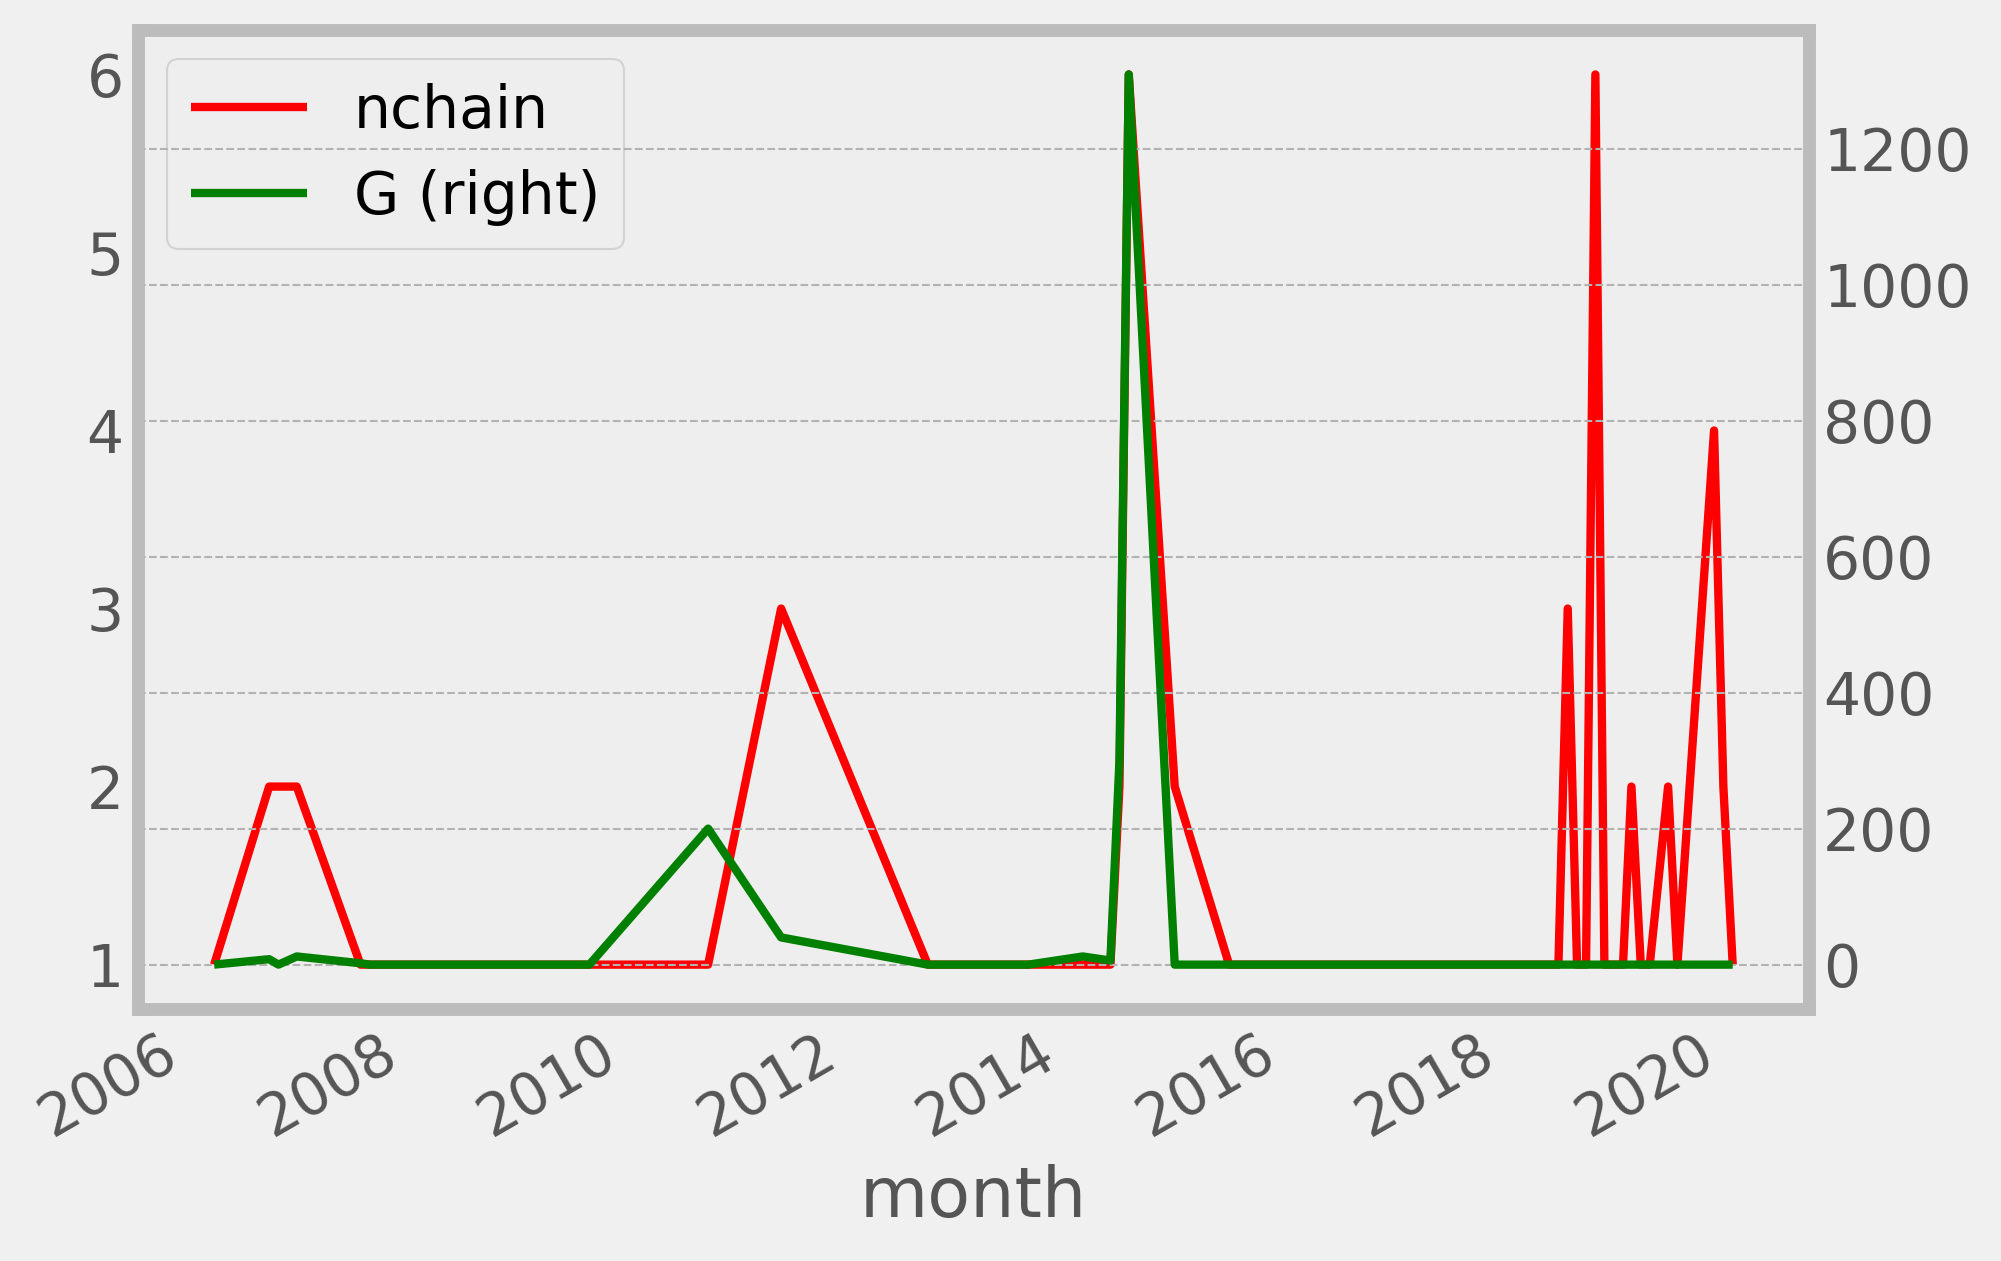
\includegraphics[width=0.7\textwidth]{./chapters/04/assets/chains_page.png}
    \caption{G and the number of chains for Barcelona page  in catalan}
    \label{fig:chainsuser}
\end{figure}

\subsection{User}
\paragraph*{wars}
sorting by mean of the lenght of the chain joined the biggest part ore from anonymous user, because
the longest chains usually are just details (like the number of championship of juve) that are
continued until somebody is blocked.

\begin{table}[H]
    \centering
    \ra{1.2}
    \begin{tabularx}{\columnwidth}{@{}Xllll@{}}
        \midrule
        \textbf{id}& \textbf{user} & \textbf{nchains} & \textbf{mean}& \textbf{nrevert}  \\ \toprule
        1 & 95.20.240.x & 7  & 60.4 & 423 \\
        2 & 95.20.242.x & 1  & 51.0 & 51  \\
        3 & 37.11.145.x & 14  & 51.0 & 714  \\
        4 & 95.20.249.x & 14  & 51.0 & 714  \\
        5 & 83.49.253.x & 1  & 47.0 & 47 \\
        
         \bottomrule
    \end{tabularx}
    
    \caption{user sorted by mean \label{table:mean}}
\end{table}

it is also possibile, given a user, to see see which are the pages in which is more active. we use
the user who made more reverts in catalan wikipedia for this example, we will call him Juan

\begin{table}[H]
    \centering
    \ra{1.2}
    \begin{tabularx}{\columnwidth}{@{}Xllll@{}}
        \midrule
        \textbf{id}& \textbf{user} & \textbf{nchains}  \\ \toprule
        1 & Marc Márquez i Alentà & 14  \\
        2 & Barcelona & 9   \\
        3 & Jocs Olímpics d'estiu de 1992 & 7   \\
        4 & Rafael Nadal i Parera & 6  \\
        5 & Catalunya &  6 \\
        6 & Lliga de Campions de la UEFA	 &  6 \\
        7 & Quim Monzó &  6 \\
        8 & Polseres vermelles &  6 \\
        9 & Jordi Sànchez i Zaragoza &  6 \\
        10 & Alfons Arús i Leita &  6\\

        
         \bottomrule
    \end{tabularx}
    
    \caption{user sorted by mean \label{table:mean}}
\end{table}
\paragraph*{monthly}
given a user we can draw his revert activity
\begin{figure}[H]
    \centering
    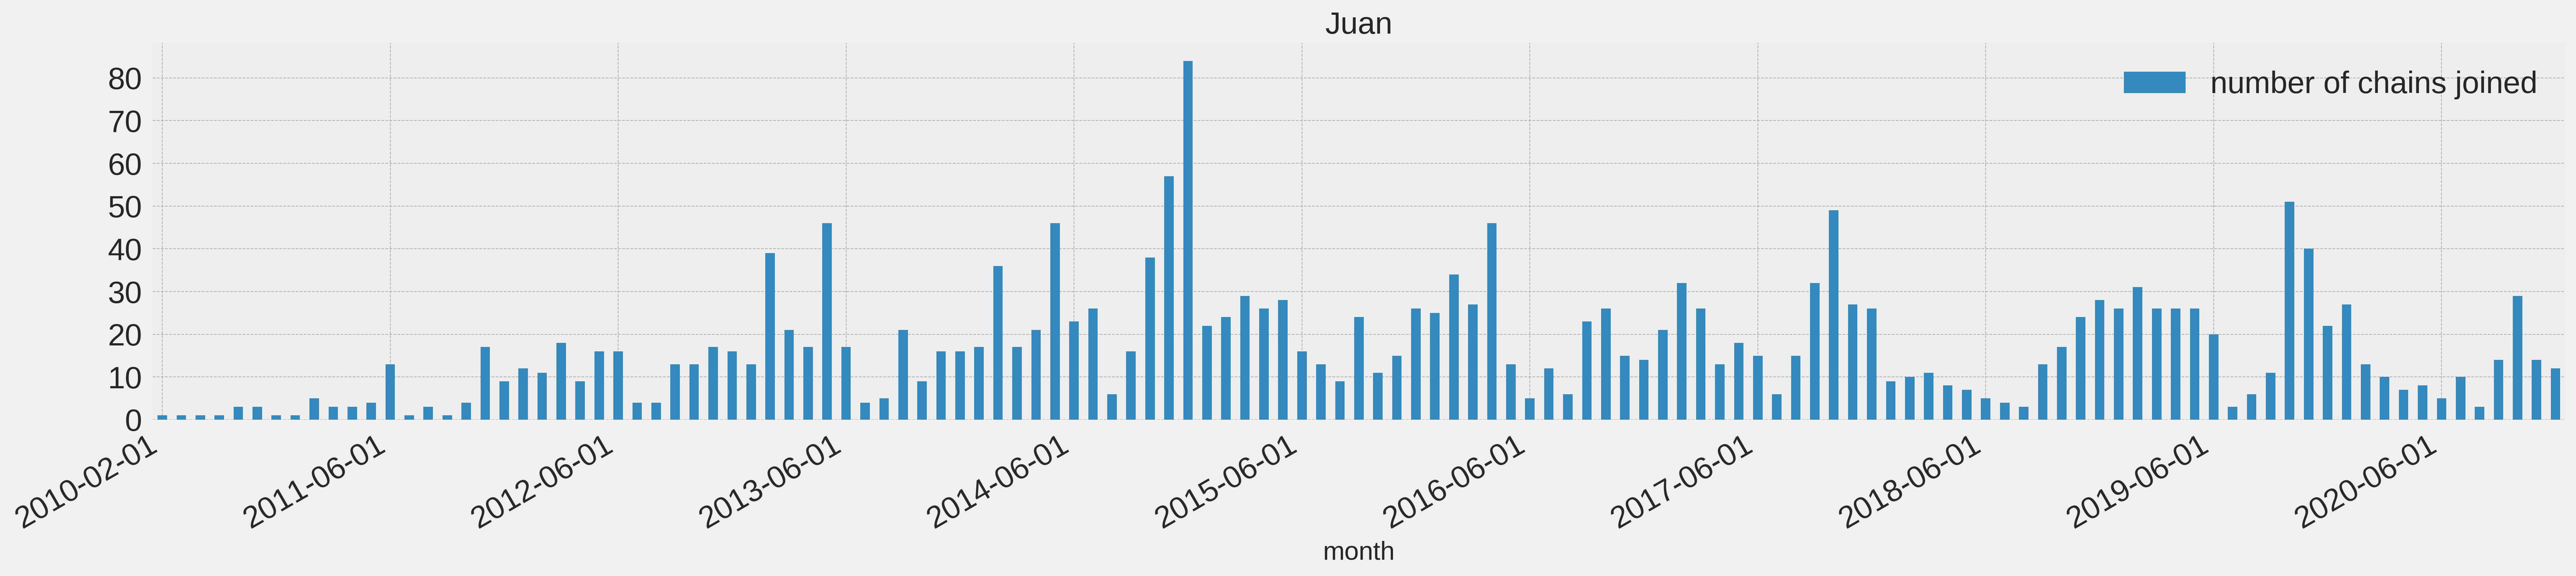
\includegraphics[width=\textwidth]{./chapters/04/assets/chains_user_month.png}
    \caption{number of chain by month of juan}
    \label{fig:chainsusermonth}
\end{figure}

\section{Group}
From the analysis of the groups we can define different ranking of pages using the number of reverts
of each group, or given a page we can plot the trend of the edits by group and detect the pages in
which admins are more interested. It is possibile for each user to say if he is target of reverts
from or if it is an admin reverted and the ration between reverted made and received. You can do so
much analysis of this data, that is the reason why it is avaiable to everyone who needs it. 

here some numbers about the users 
\begin{table}[H]
    \centering
    \ra{1.2}
    \begin{tabularx}{\columnwidth}{@{}Xrrr@{}}
        \midrule
        \textbf{len}& \textbf{registered} & \textbf{admin}& \textbf{active}  \\ \toprule
        en& 41,825,139& 1,089& 127,566  \\
        es & 6'266'812 & 69 & 16'143   \\
        it & 2'140'498 & 114 & 8'208\\
        ca & 391'067 & 22 & 1'180   \\
     

        
         \bottomrule
    \end{tabularx}
    
    \caption{user sorted by mean \label{table:statsuser}}
\end{table}

\subsection{Page}
\paragraph*{reverts}
we can see how the influence of admin is higher in the italian wikipedia stagionaloty
\begin{figure}[H]
    \centering
    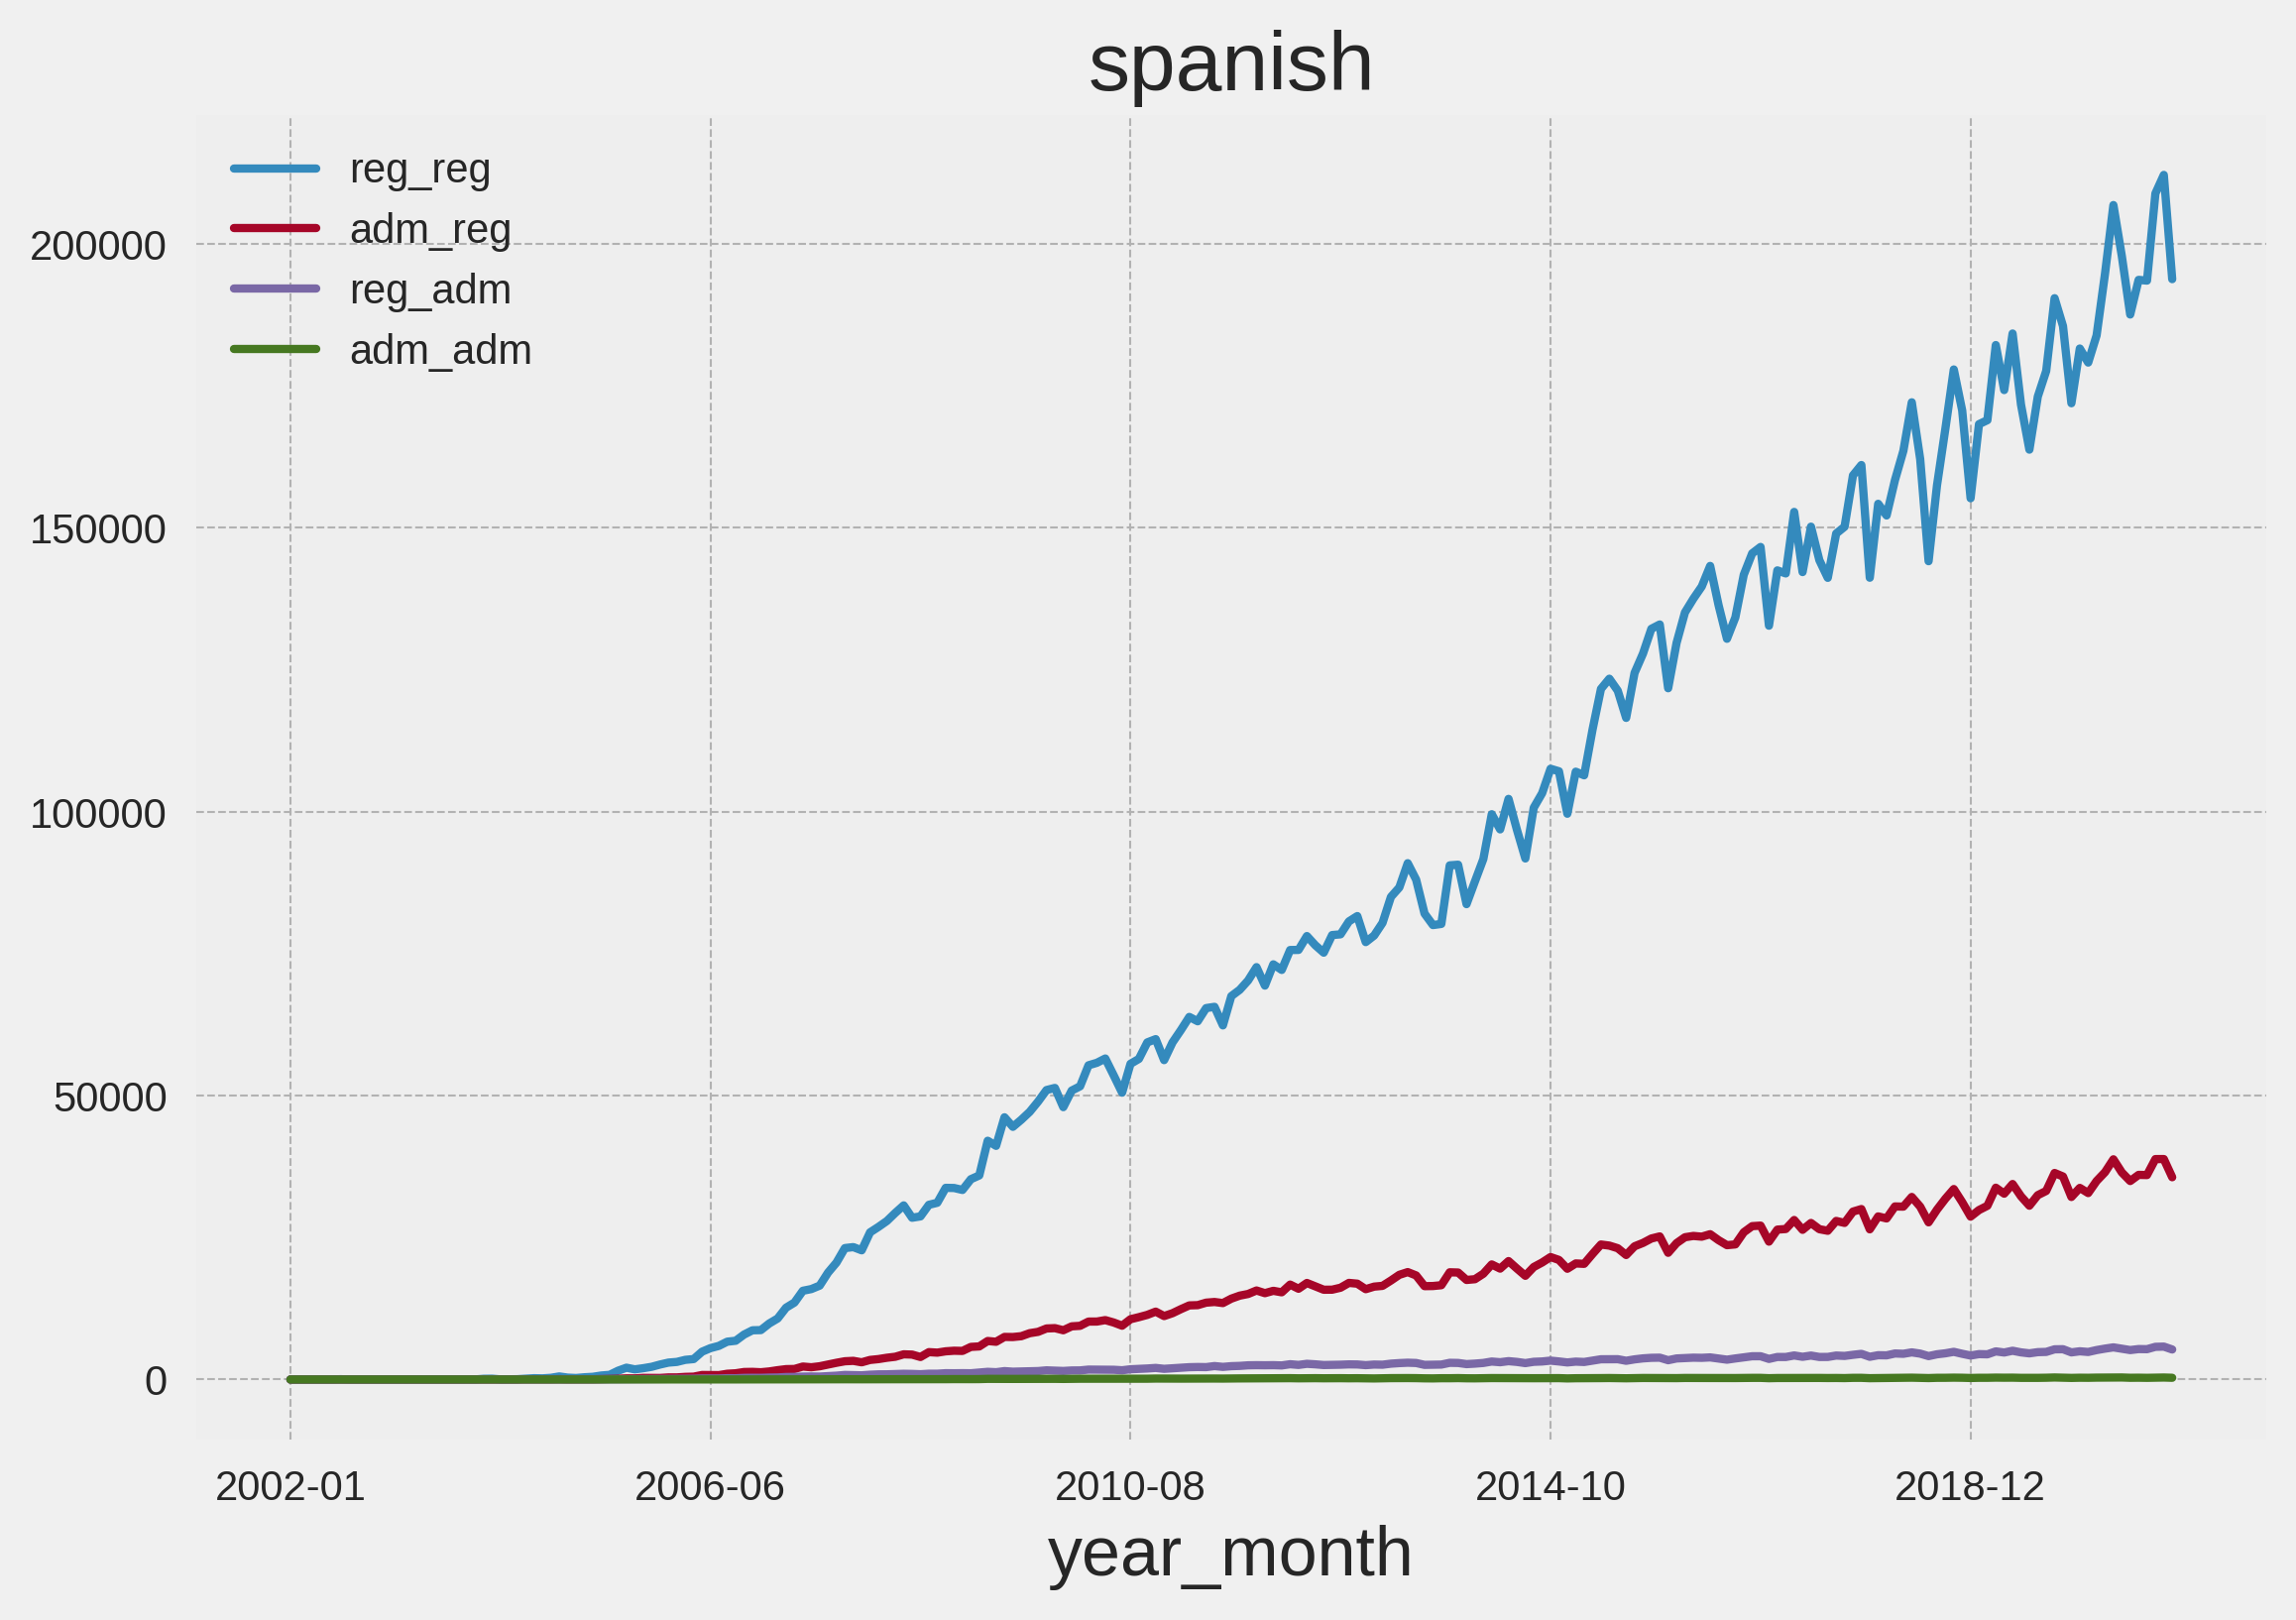
\includegraphics[width=0.45\textwidth]{./chapters/04/assets/admin_es.png}
    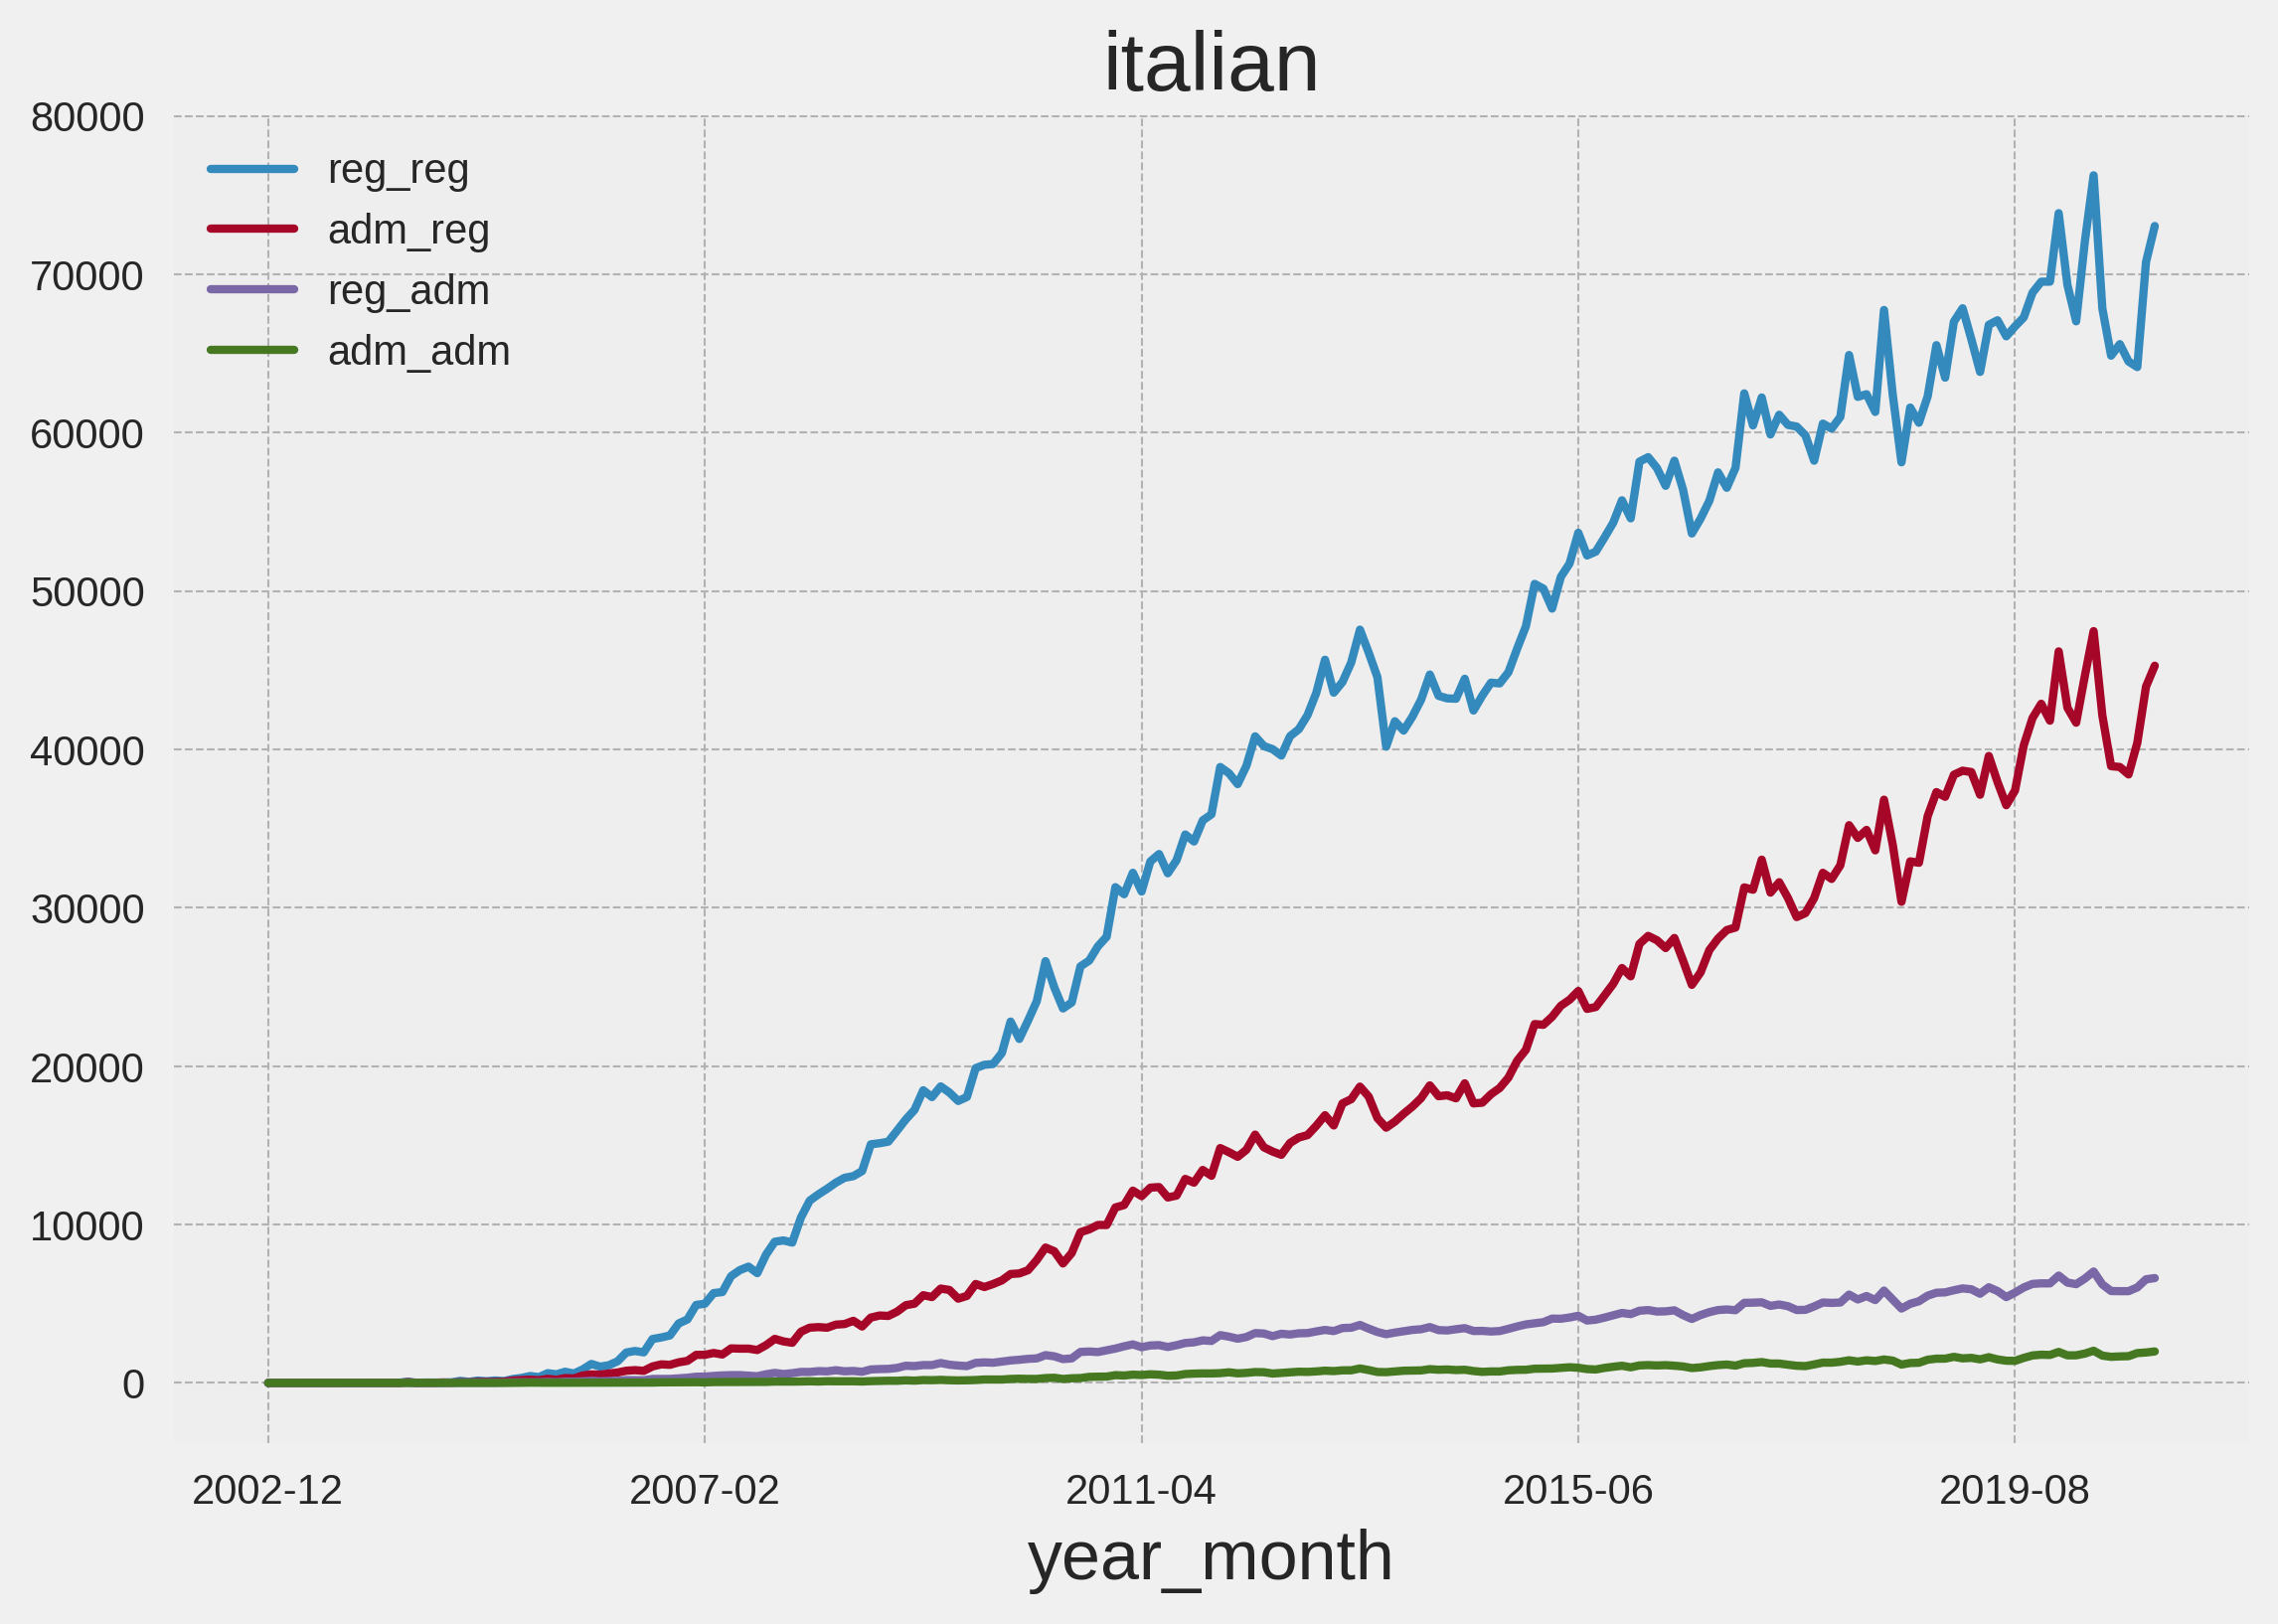
\includegraphics[width=0.45\textwidth]{./chapters/04/assets/admin_it.png}
    \caption{number of chain by month of juan}
    \label{fig:compare}
\end{figure}
\paragraph*{mutual}
\subsection{User}
\paragraph*{reverts}
the plots represents, for italian, catalan and spanish, the number of revert done and received by
each category, we can see how the behaviour of the users changes with the languages especially
towards admins. for reverts done italian and spanish are similar, but the share of the reverts of
the admin in the received one is very different. in italy the reverts received are equally devided
between anonymous and registered 
\begin{figure}[H]
    \centering
    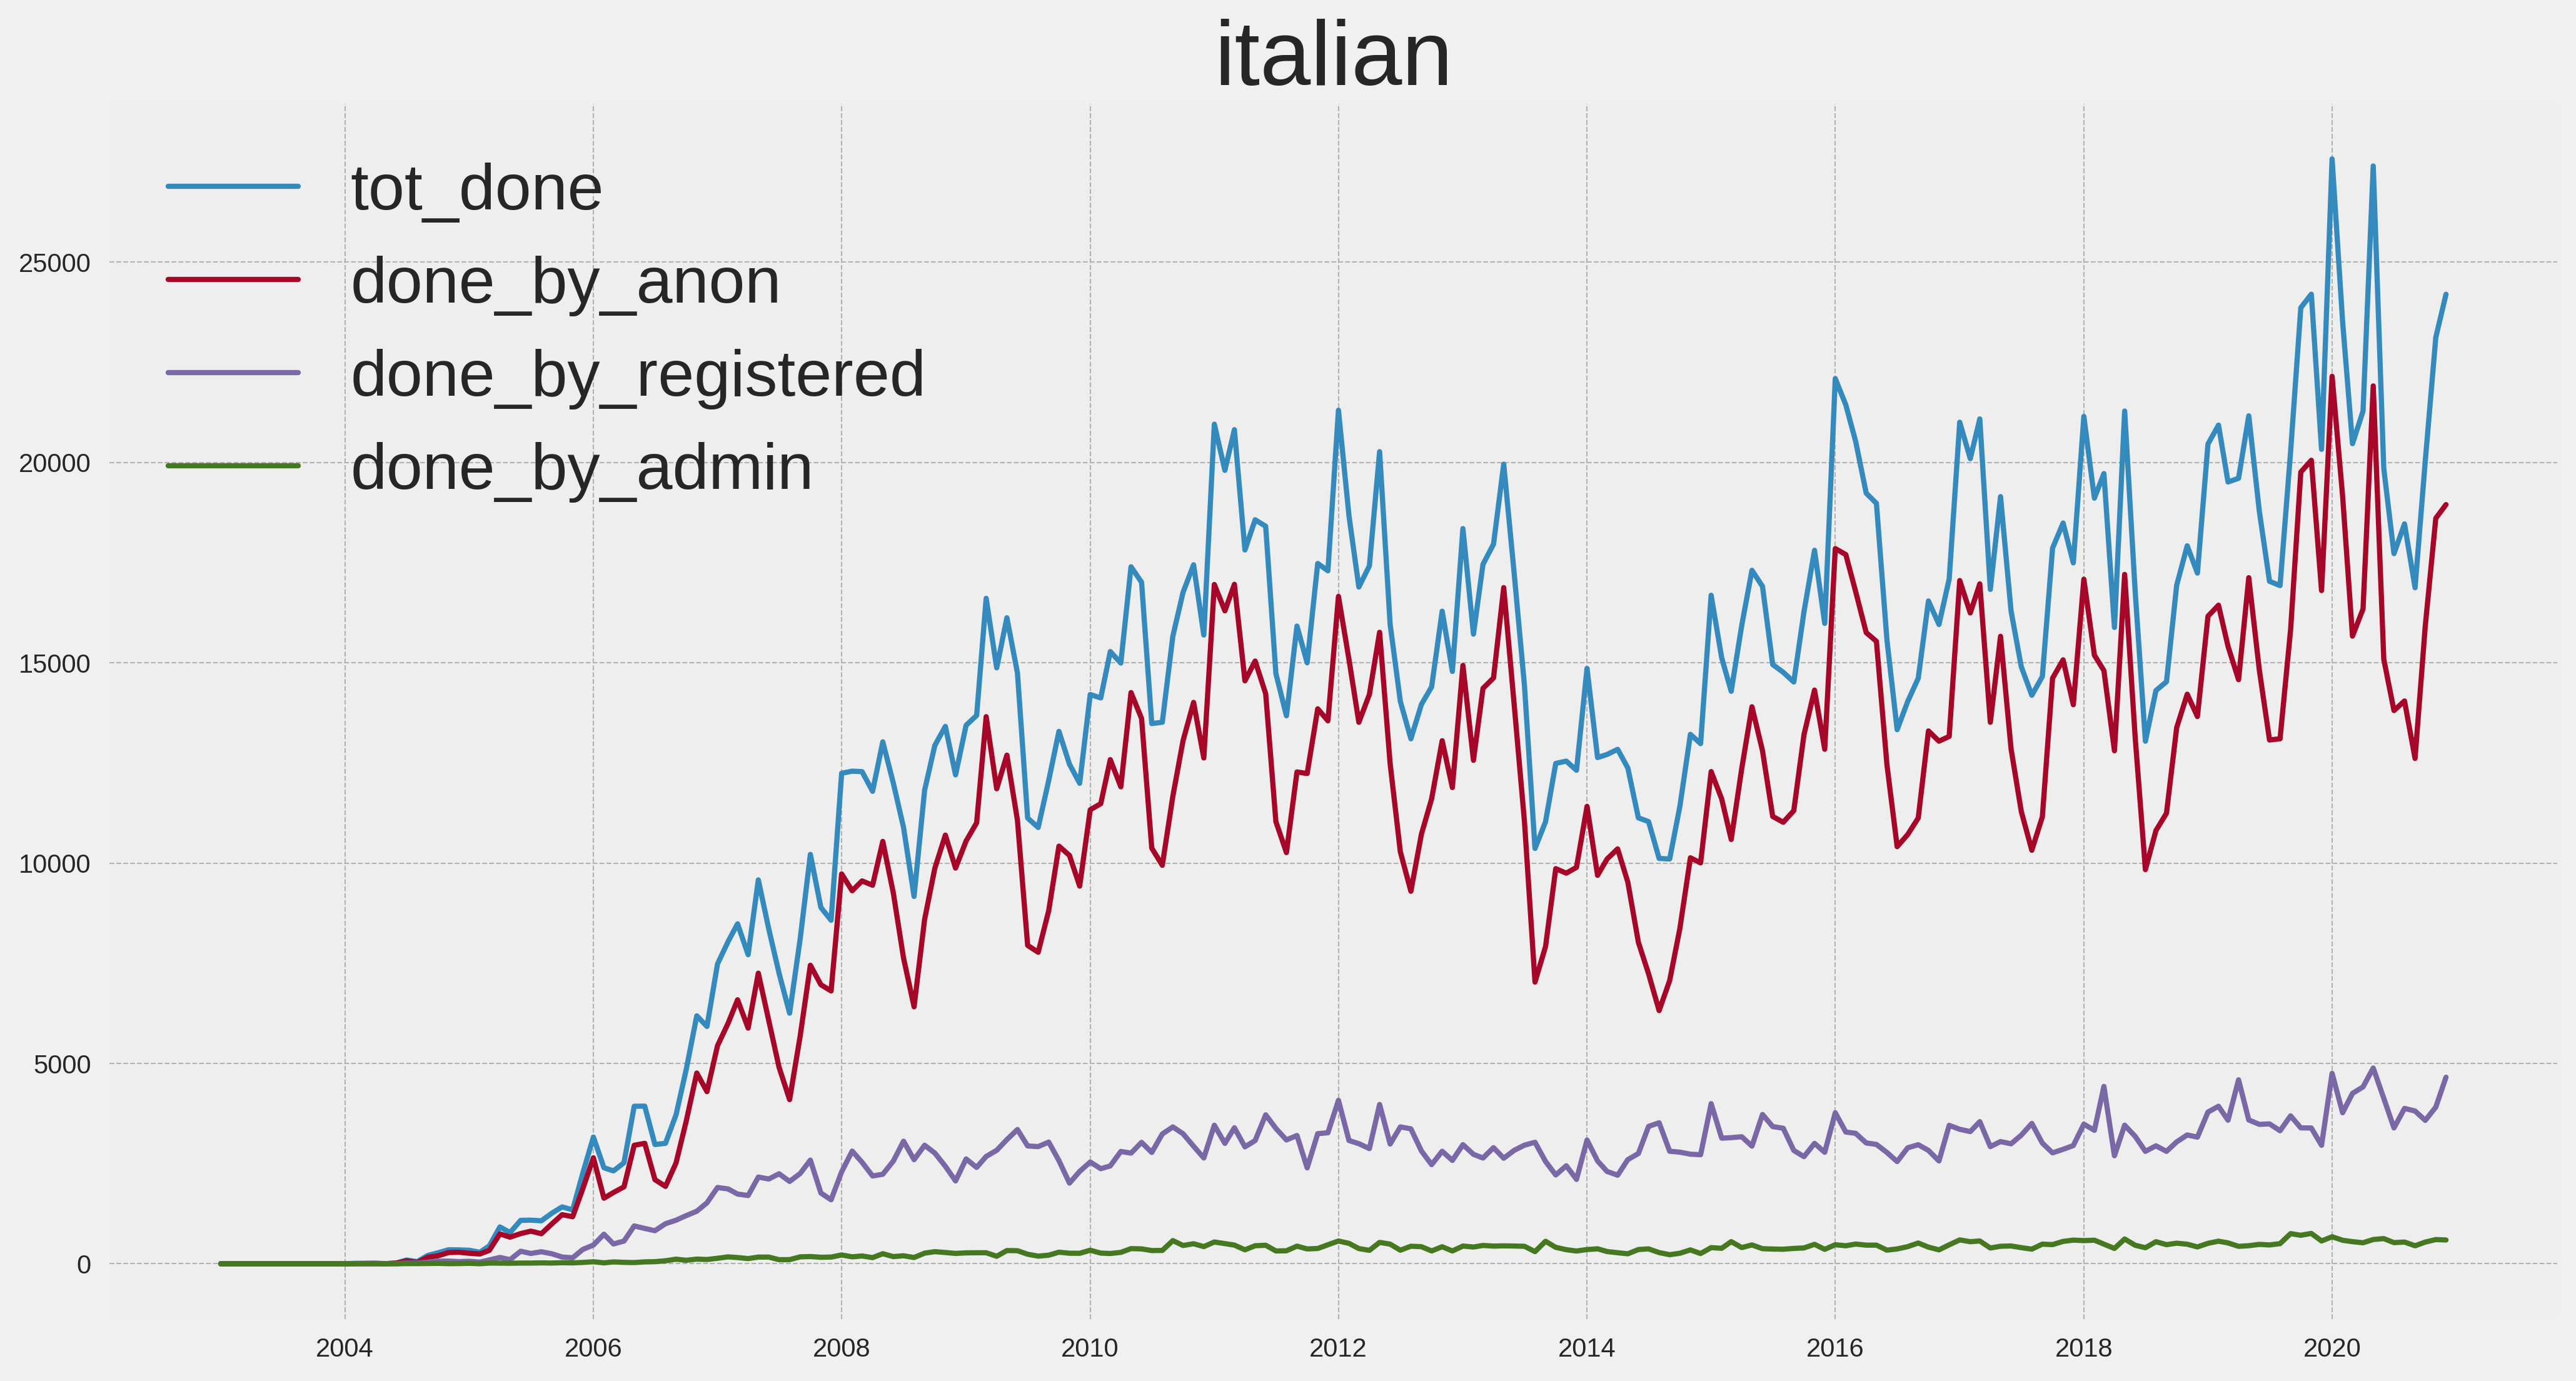
\includegraphics[width=0.49\textwidth]{./chapters/04/assets/revert_done_it.png}
    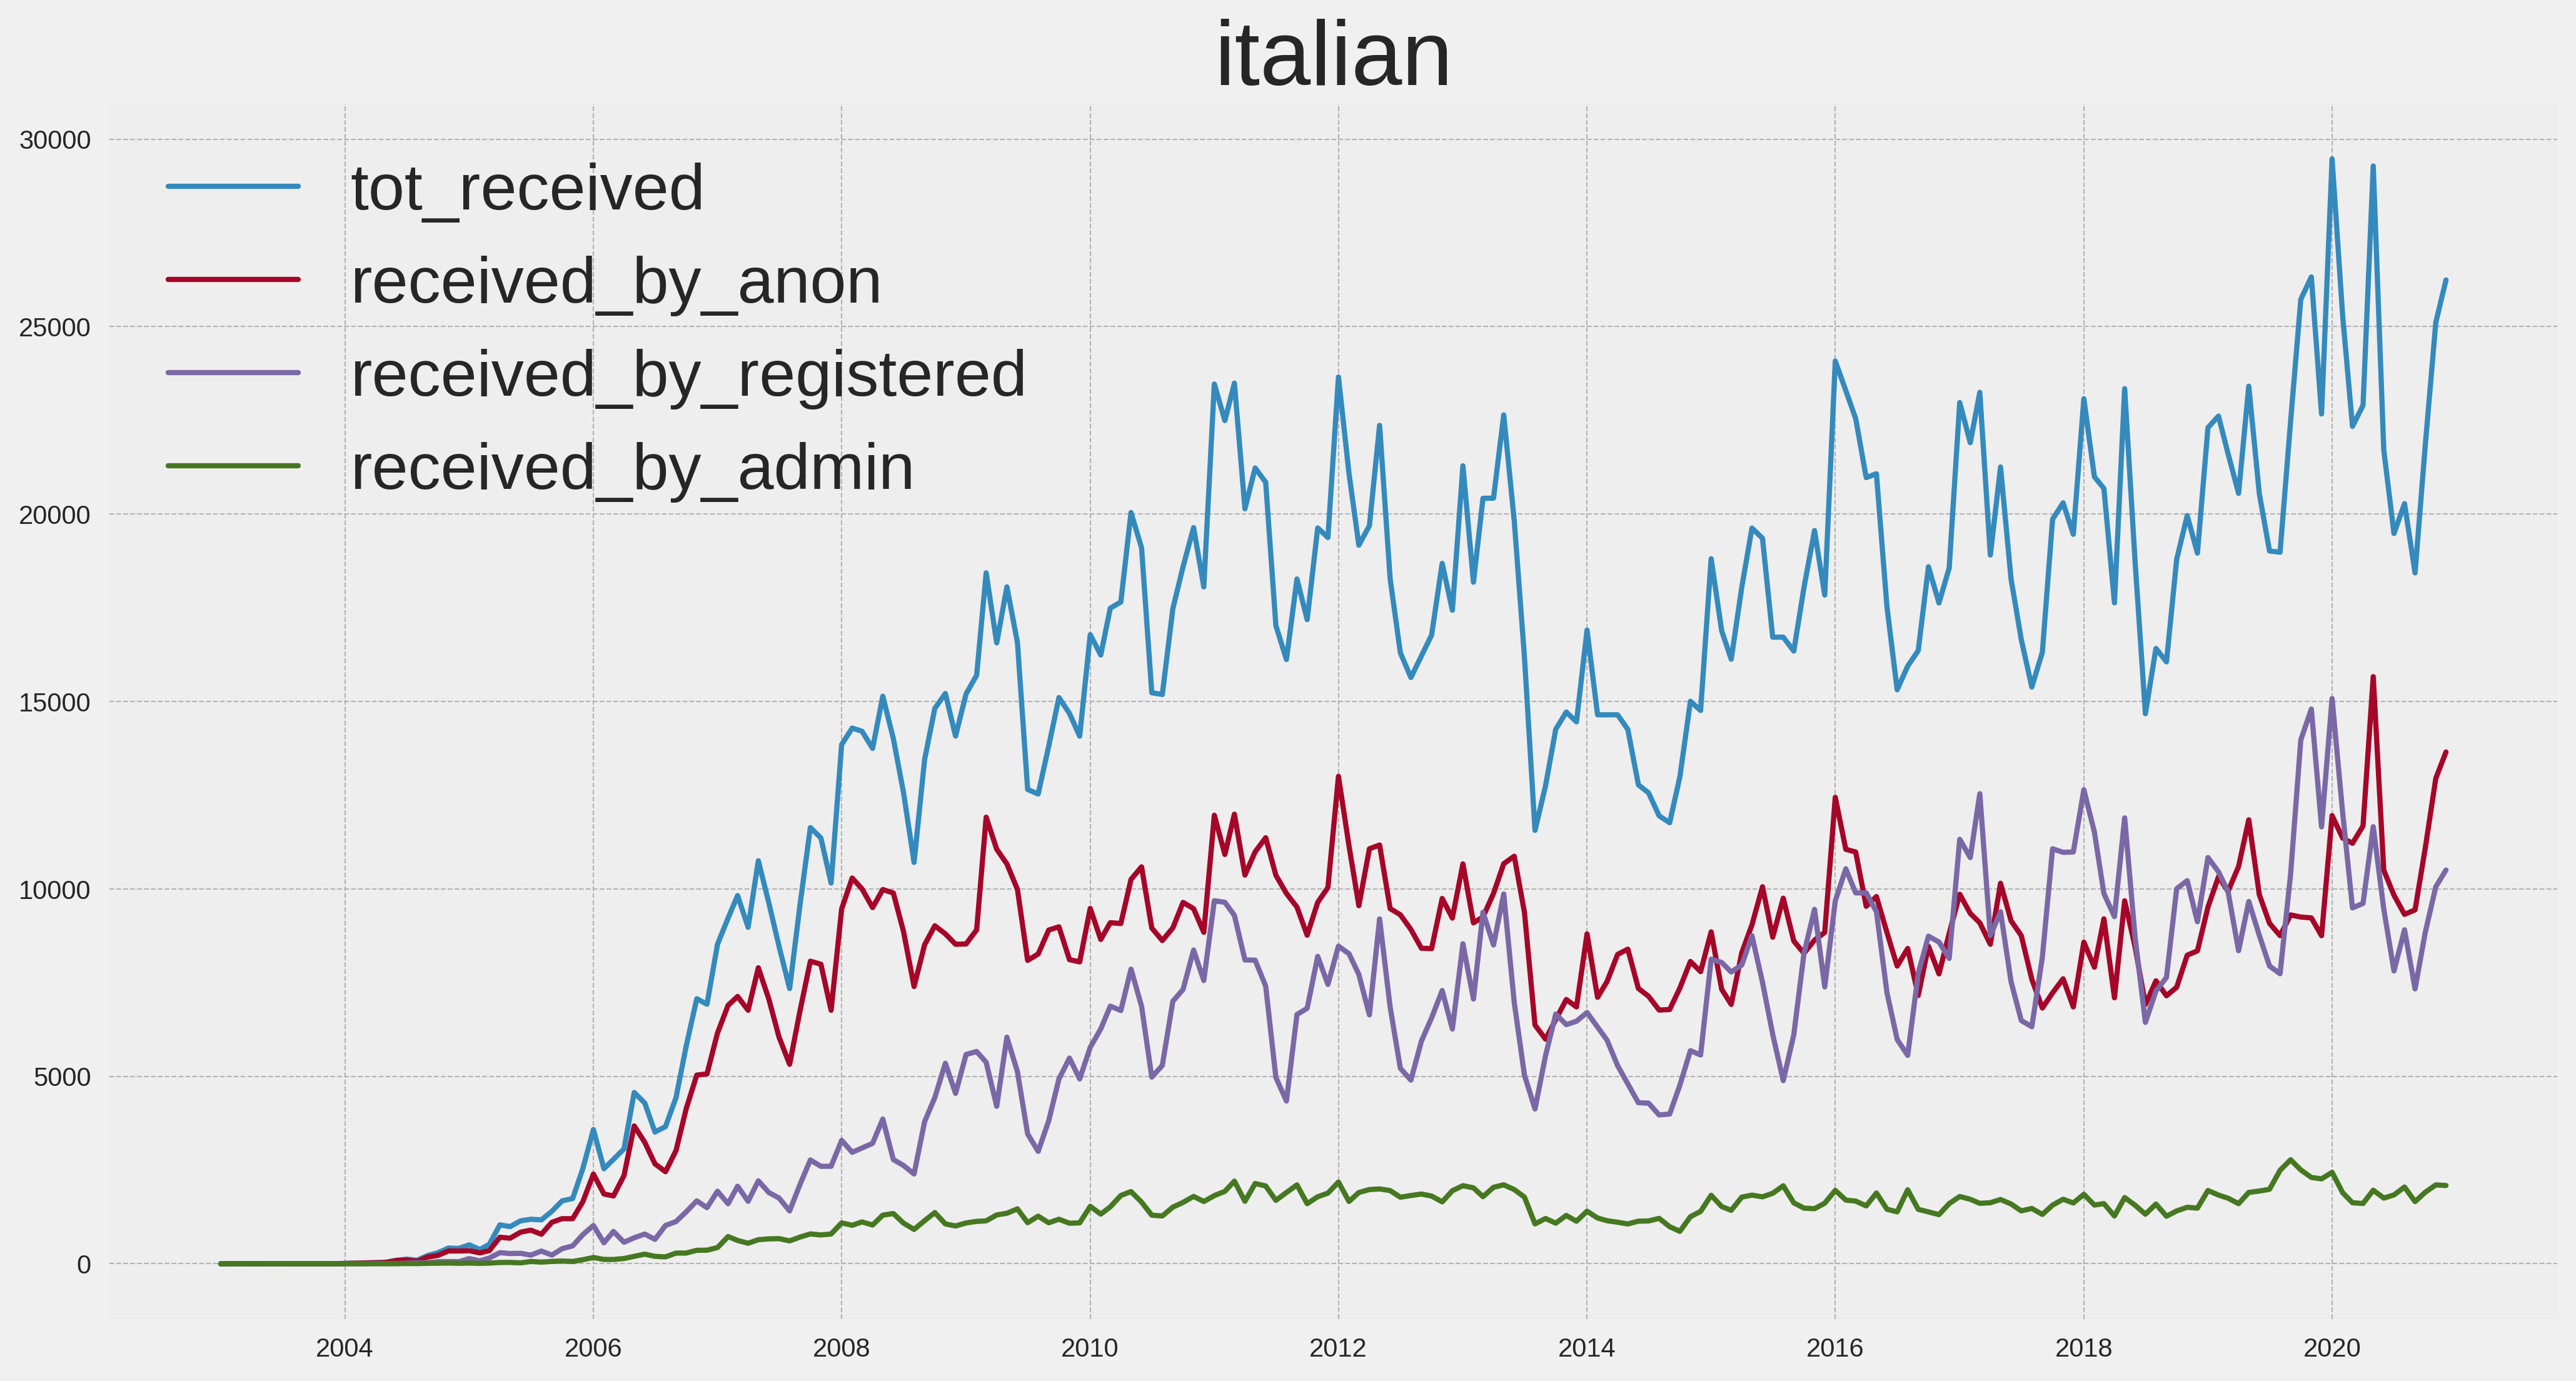
\includegraphics[width=0.49\textwidth]{./chapters/04/assets/revert_received_it.png}
    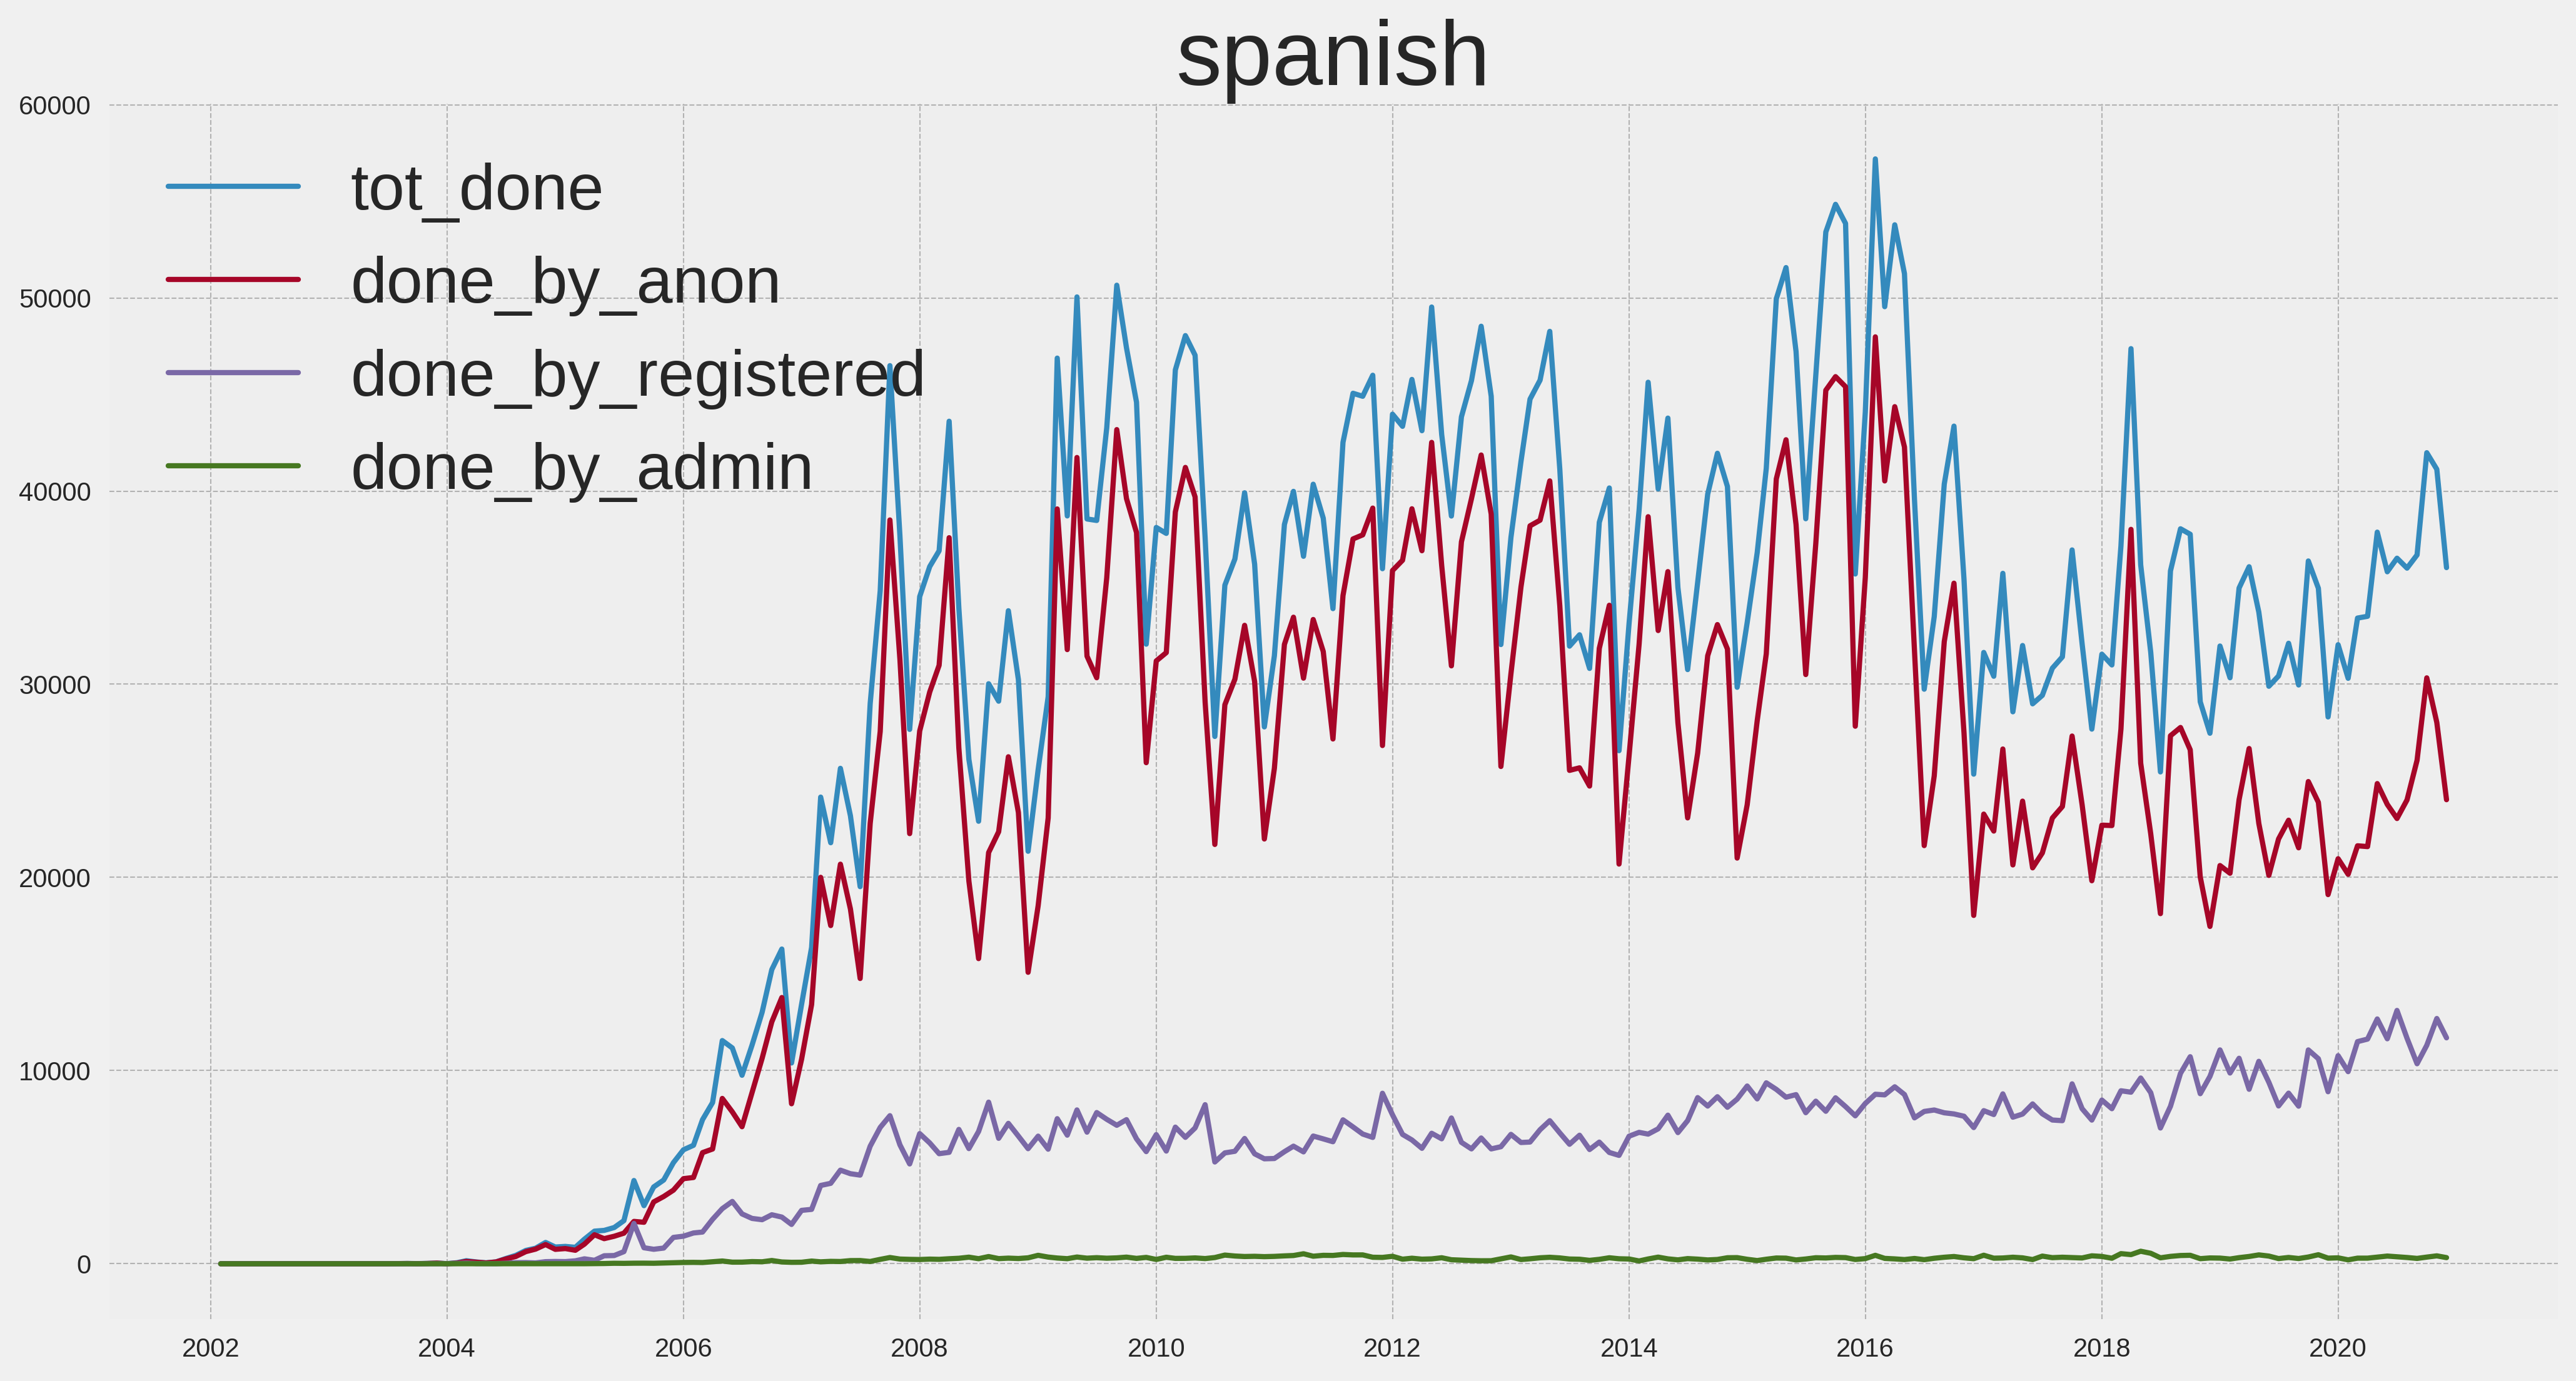
\includegraphics[width=0.49\textwidth]{./chapters/04/assets/revert_done_es.png}
    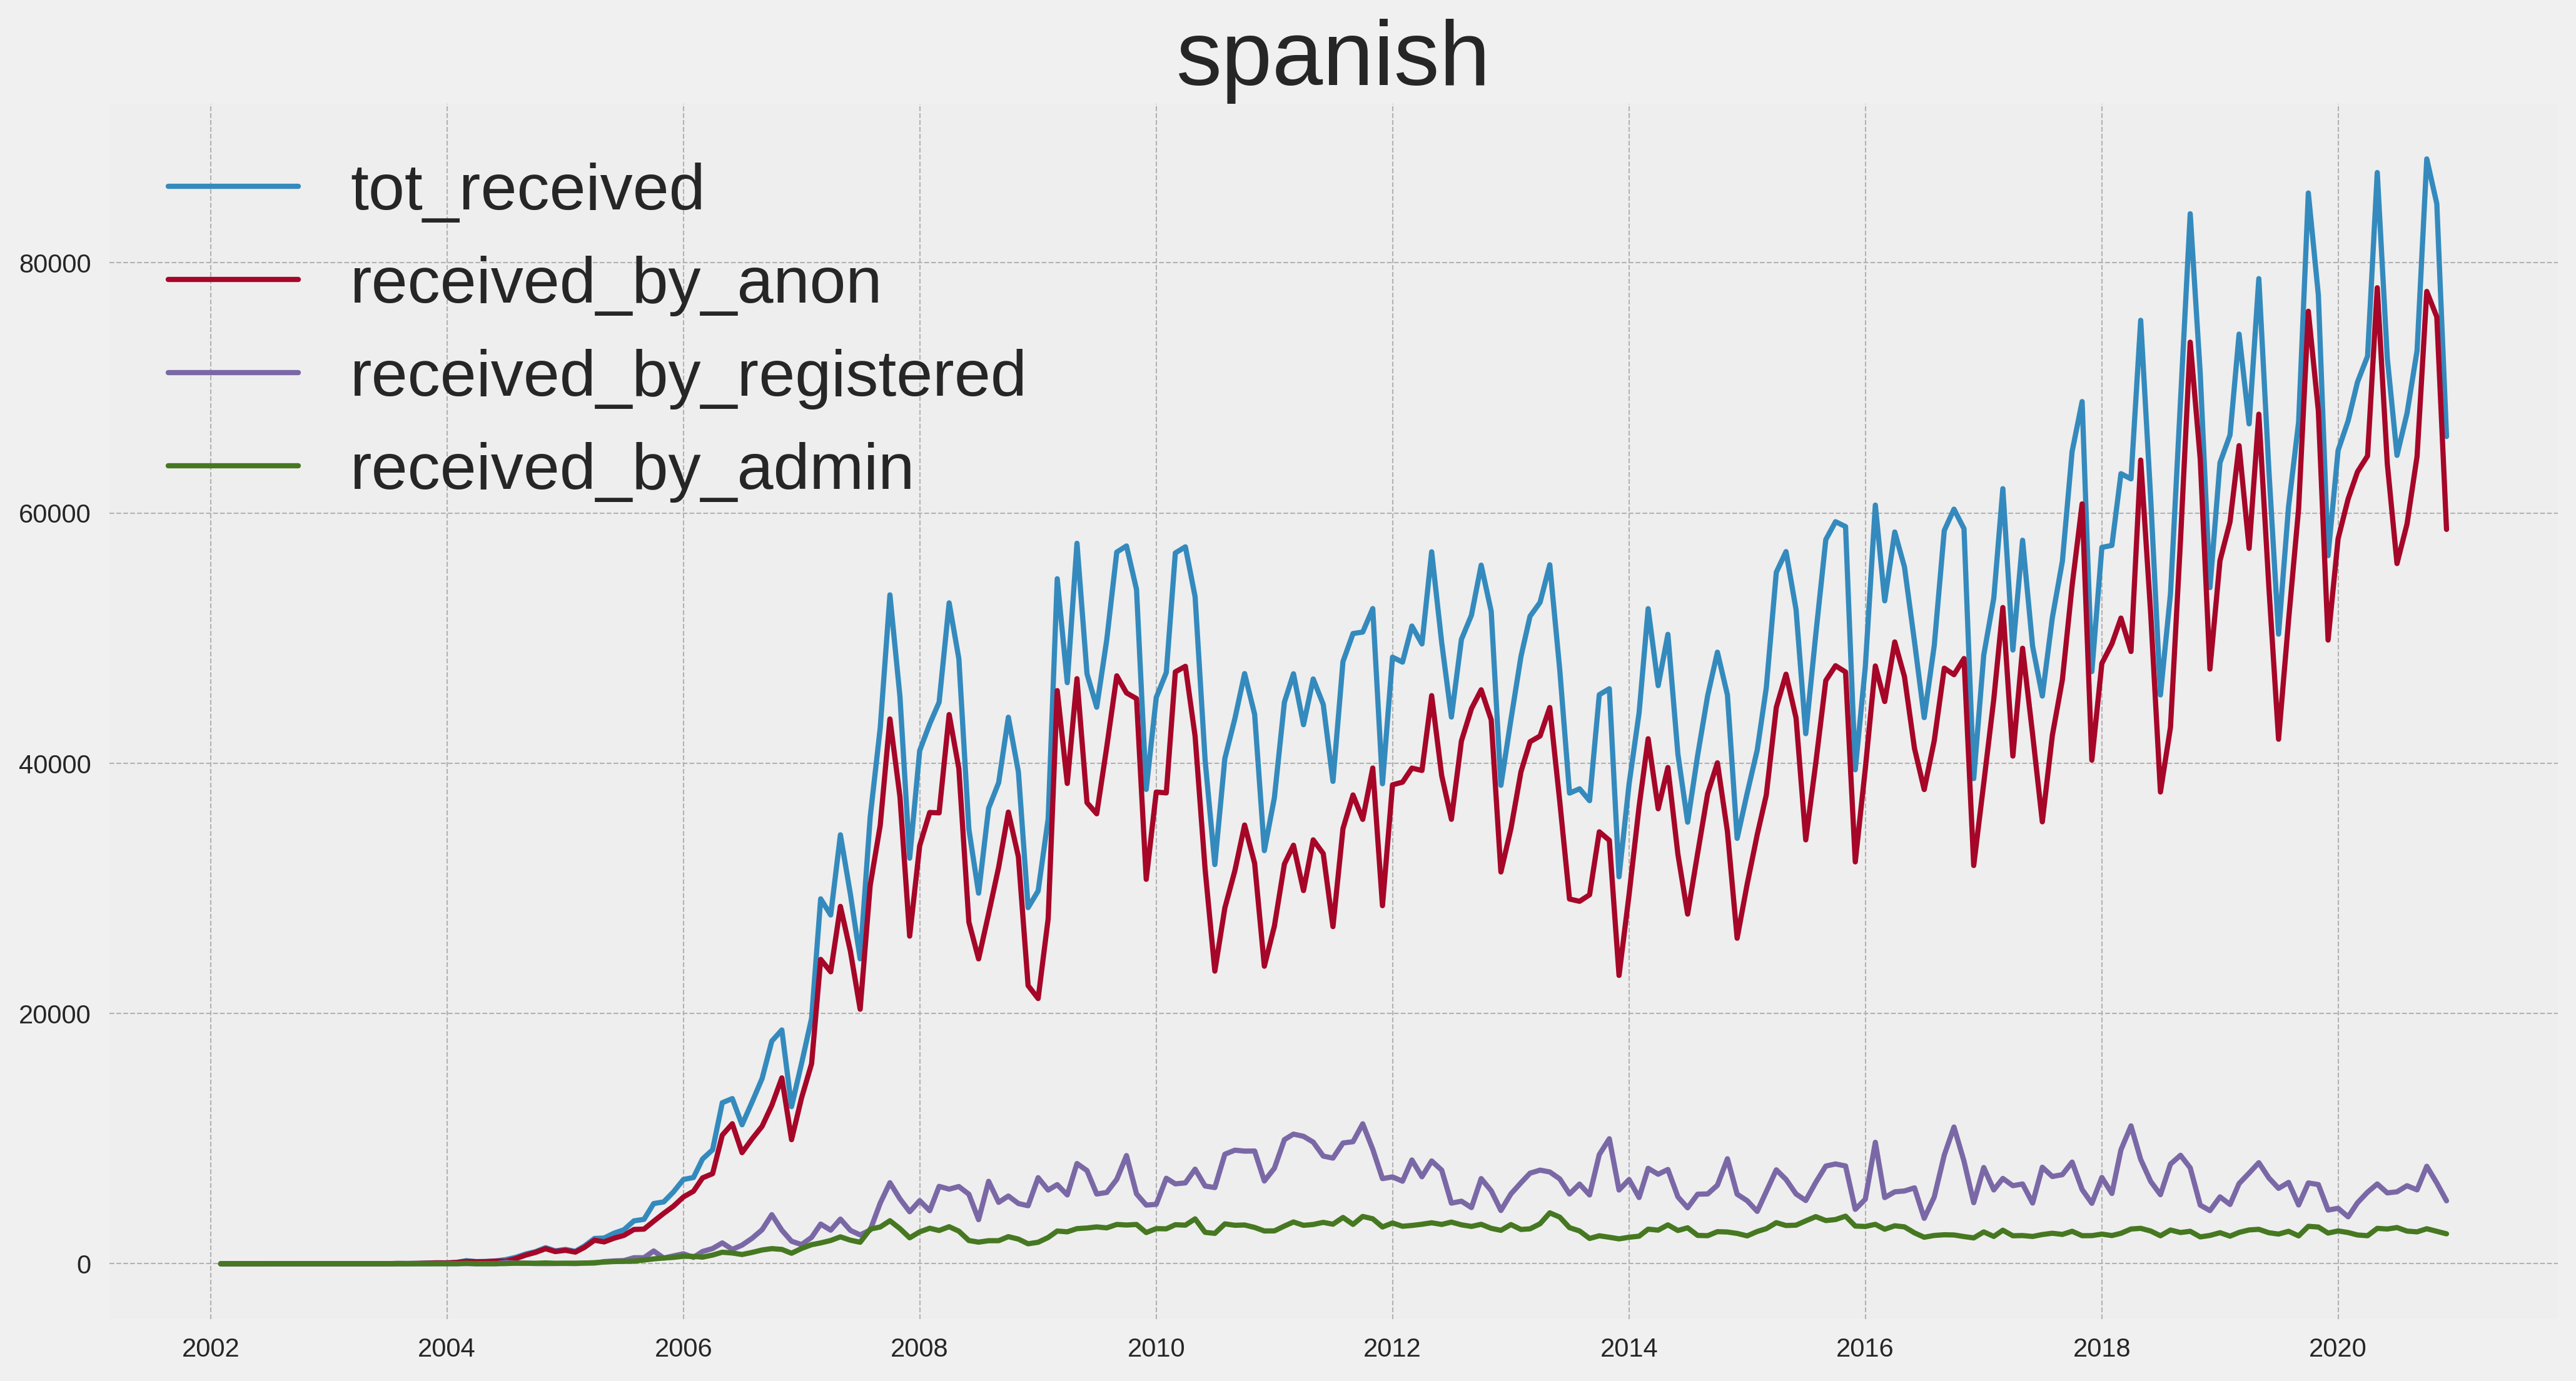
\includegraphics[width=0.49\textwidth]{./chapters/04/assets/revert_received_es.png}
    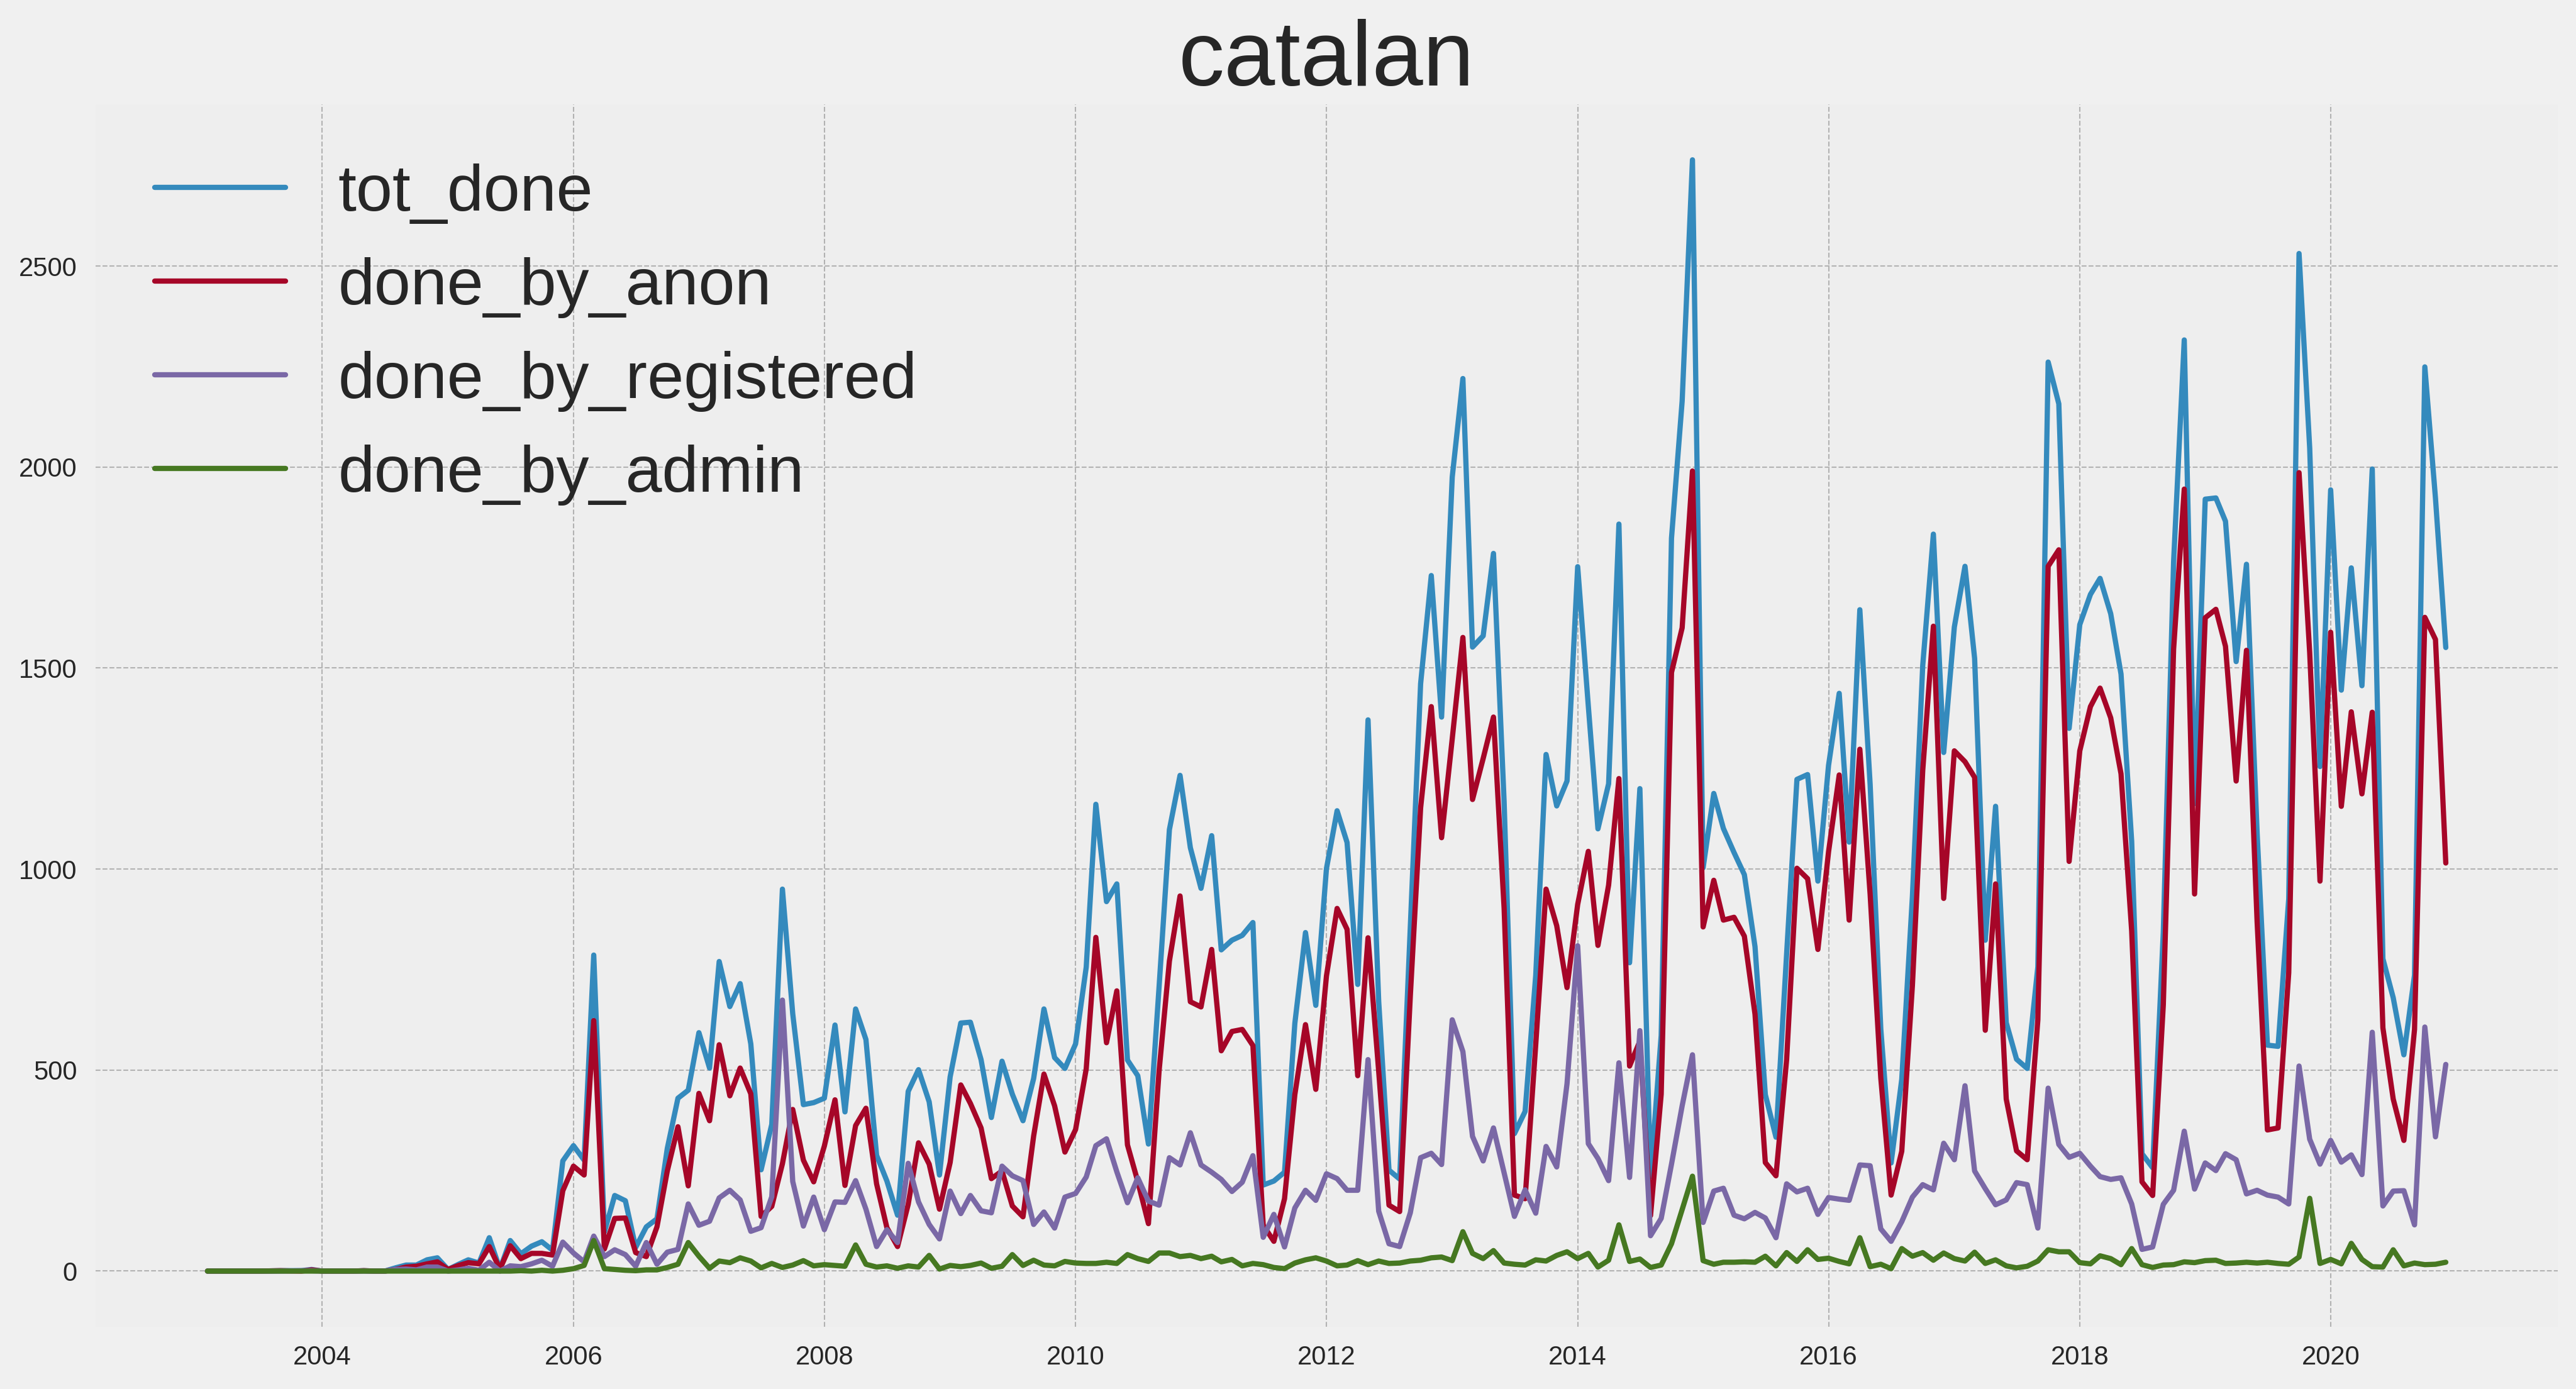
\includegraphics[width=0.49\textwidth]{./chapters/04/assets/revert_done_ca.png}
    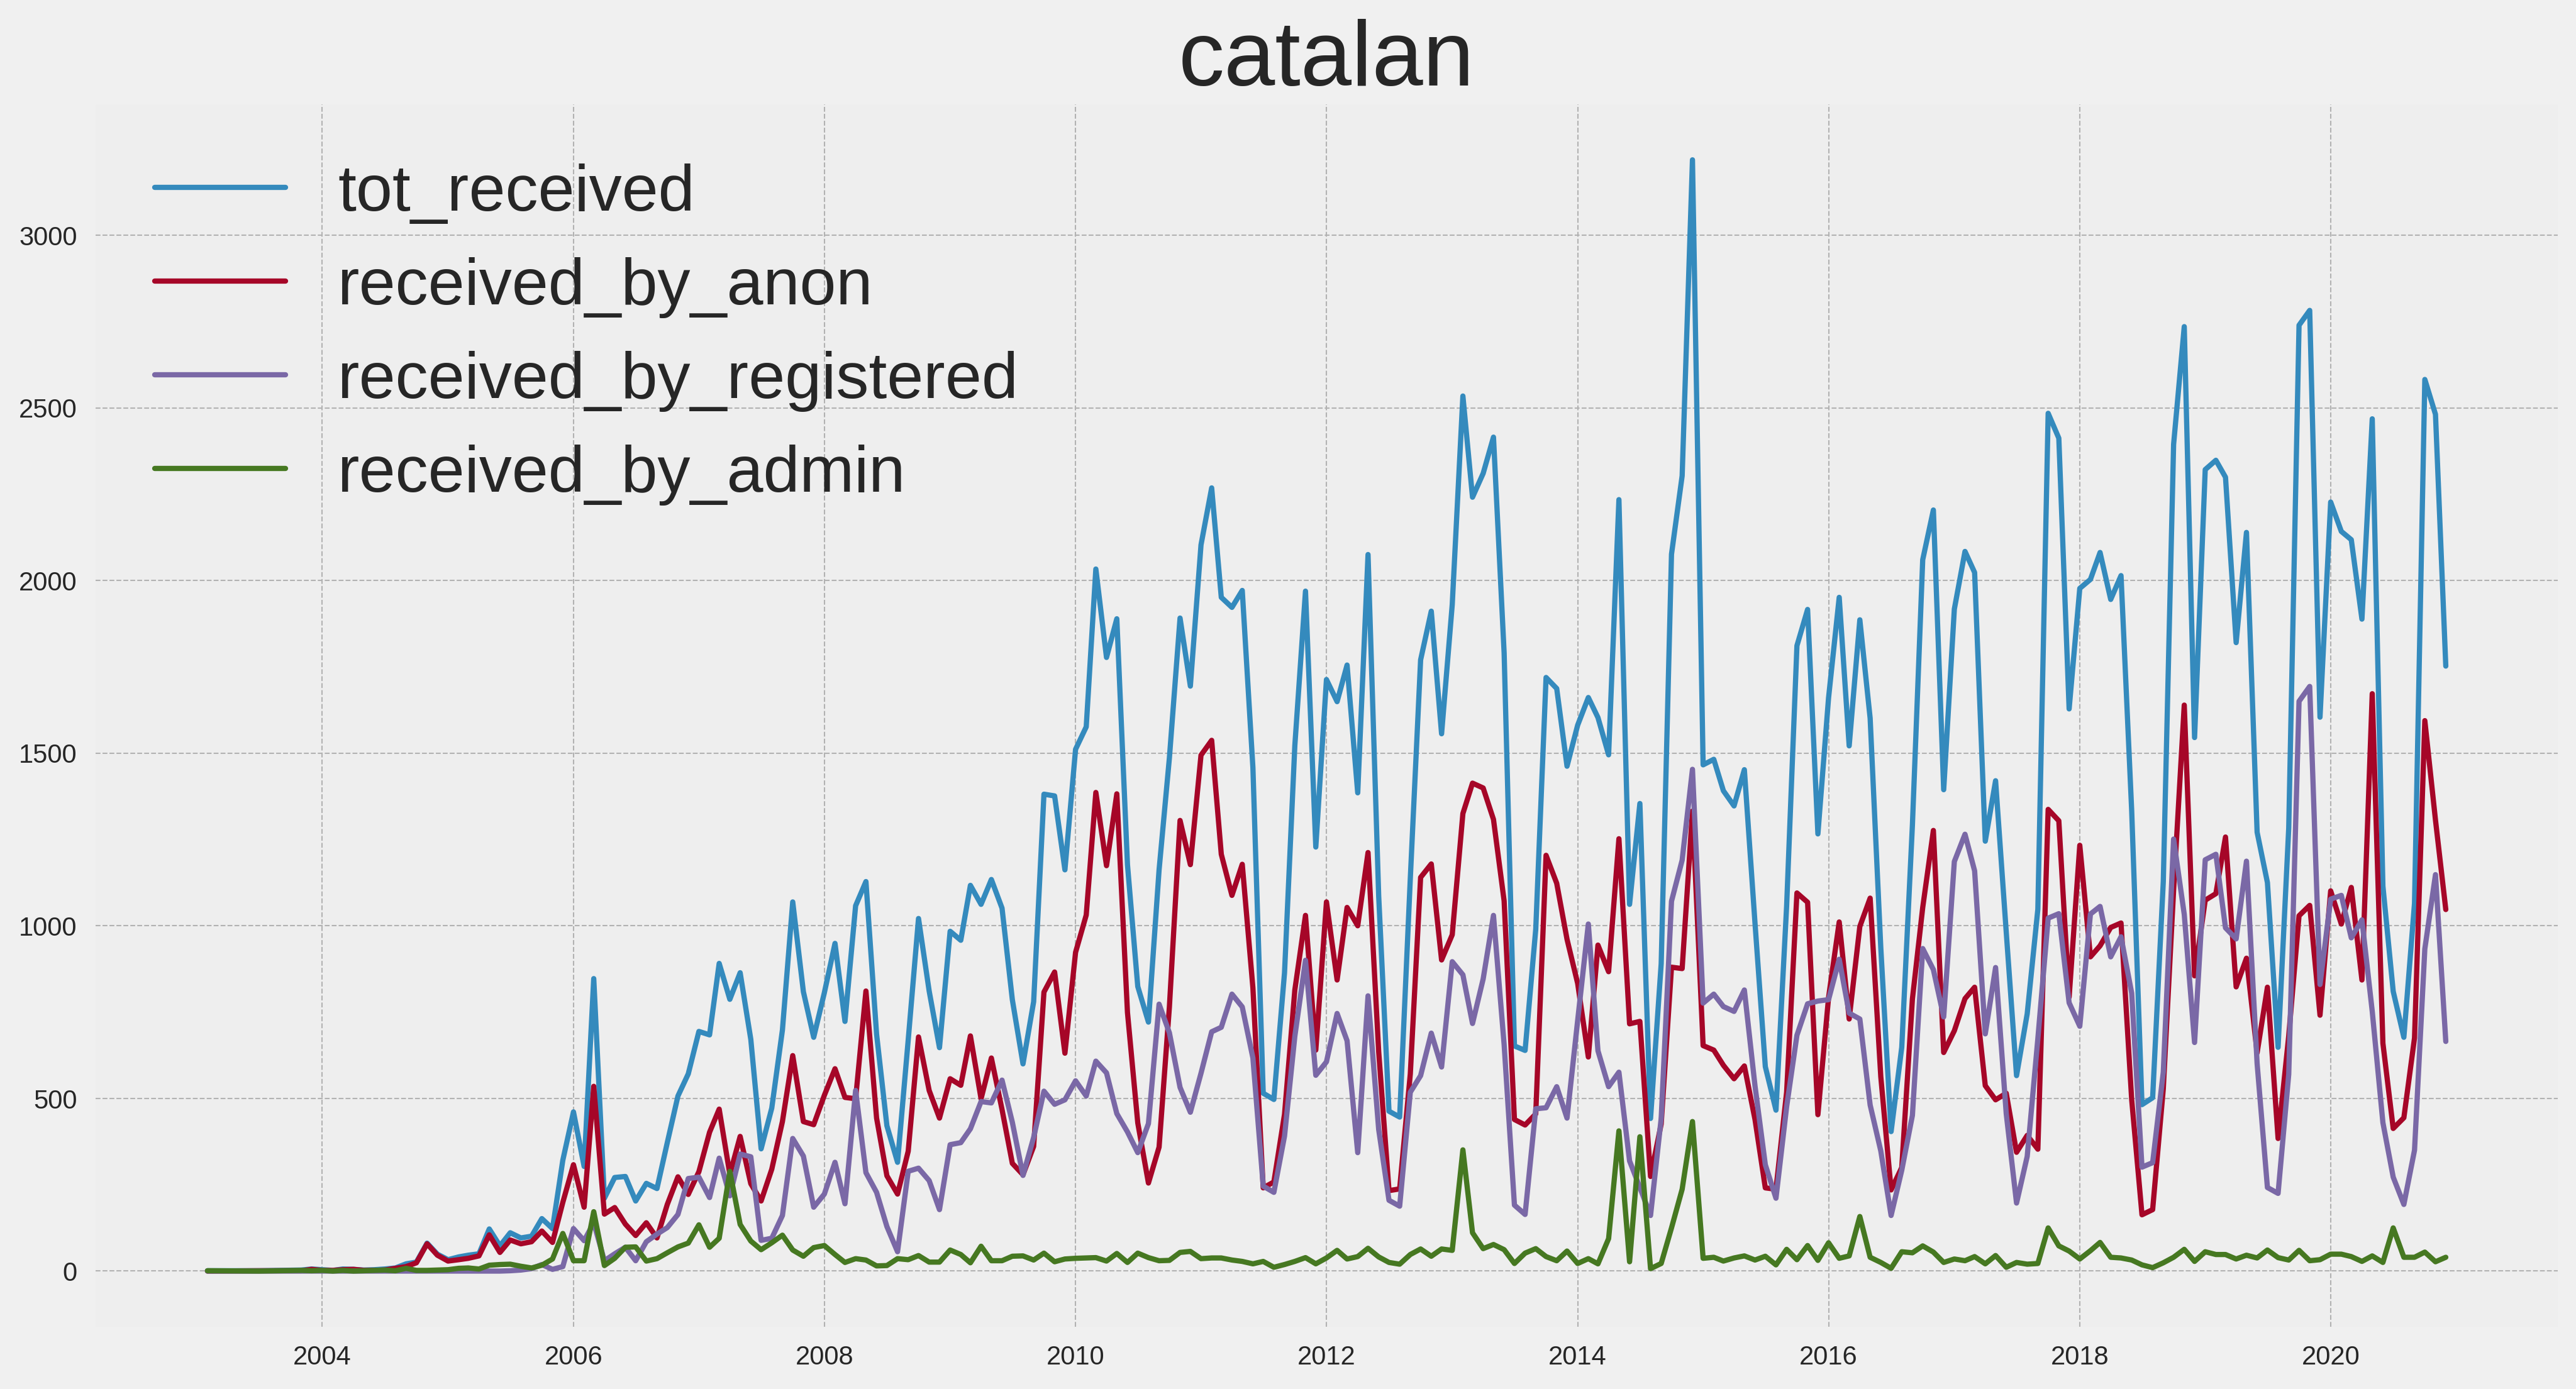
\includegraphics[width=0.49\textwidth]{./chapters/04/assets/revert_received_ca.png}
    \caption{number of chain by month of juan}
    \label{fig:revuser}
\end{figure}
\paragraph*{mutual}






